%=====================================================================
%  How much validation is enough?
%  Budget sensitivity of algorithm selection in lightweight link prediction
%
%  Target venue: The Computer Journal (Oxford University Press).
%  NOTE ON THE CLASS: comjnl.cls in this directory is a LOCAL SHIM that
%  reproduces the journal's interface; the official class is distributed
%  by OUP and was not reachable from this machine.  At submission, delete
%  comjnl.cls, add the official comjnl.cls + compj.bst, and switch the
%  bibliography style to compj (see docs/SUBMISSION_GUIDE.md).
%
%  Compile from this directory:
%    pdflatex main ; bibtex main ; pdflatex main ; pdflatex main
%  Tables are generated by scripts/analyze_results.py and live in ../tables;
%  figures are generated by scripts/make_figures.py and live in ../figures.
%=====================================================================
\documentclass{comjnl}

\usepackage{subcaption}
\usepackage{multirow}
\usepackage{array}
\usepackage{url}

\graphicspath{{../figures/}}

\title[Validation budget and sampler]{How much validation evidence does an index selection need?
Budget, sampler and the plateau in link-prediction benchmarks}

\author{Junkai Fan}
\affiliation{School of Business Administration, Northeastern University,
Shenyang 110167, China}
\email{fanjk@mails.neu.edu.cn}
\orcid{0009-0006-9624-385X}

\shortauthors{J. Fan}

\received{7 November 2026}
\revised{7 November 2026}

\keywords{link prediction; model selection; validation budget; negative
sampling; benchmarking methodology; performance estimation}

\begin{document}
\maketitle

\begin{abstract}
\noindent
Link-prediction papers choose a similarity index on a validation sample of non-edges and
report the winner on a held-out test set, but neither the size of that sample nor the
negative sampler that produced it is defended. We measure both decisions on twenty-three
networks, ten distinct indices, seven validation budgets from 20 to 2{,}000 balanced pairs
and three negative-sampling regimes, 9{,}660 selections in all. Mean selection loss falls
from 0.0156 to 0.0034 AUC and flattens after a few hundred pairs; its median is zero, so
the plateau is a tail of near-tied cases rather than a level every study pays. A near-tie
theory predicts the decay exponent, $\gamma=\beta(1+\alpha)=0.74$--$0.79$, from a measured
noise decay of $\beta=0.55$--$0.62$, and attributes only 7--22\% of the residual at
2{,}000 pairs to validation noise. The larger risk sits in the construction of the
evidence: validating on uniform negatives and deploying on two-hop negatives can cost up
to 0.073 AUC, against 0.004 for the matched design. Five selection rules and sequential
racing fail to beat a single draw of the same size, and hedging across regimes recovers
86\% of the two-hop penalty only when the deployment regime is among those averaged,
2--12\% otherwise. We release a planning tool that estimates the required budget from a
small pilot and recommend that studies report the validation budget, the sampler and the
runner-up scores.
\end{abstract}


\section{Introduction}

Link prediction asks which unobserved pairs of vertices are likely to become connected. It is the computational core of friend and follower recommendation, of candidate generation in biological interaction screens, and of the reconstruction of partially observed infrastructure and citation networks \citep{guimera2009missing,lu2015toward}. Most public benchmarks still lack node attributes, and for them the standard tool set is a family of local similarity indices that score a pair by counting or weighting its common neighbours \citep{libennowell2007link,lu2011link}. A typical empirical paper evaluates a handful of such indices on a validation sample of non-edges, selects the one with the highest area under the receiver operating characteristic curve (AUC), and reports that index on a disjoint test sample. The selection step is treated as bookkeeping.

It is not bookkeeping. Choosing the best of $k$ candidates from a finite sample is a model-selection problem, and the winner of that comparison is biased upwards relative to its true performance---the optimizer's curse \citep{smith2006optimizer} or winner's curse. Two quantities are therefore conflated in the usual reporting: the test performance of the selected index, and the test performance of the index that would have been selected with complete knowledge. The difference between them is the price of the selection decision, and it depends on how much validation evidence was available.

The distinction matters because validation evidence in link prediction is unusually cheap to vary and unusually rarely reported. Edges can be held out in any quantity; non-edges can be sampled in any quantity; and nothing in the usual experimental narrative fixes the size of the validation sample. Papers that compare ten indices on a network of a few thousand edges routinely draw a few hundred validation pairs, and papers that compare two indices routinely draw many more, without either choice being defended. If the amount of evidence changes the identity of the winner, then the reported winner is partly an artefact of an unreported decision.

Learning-curve research in machine learning has long studied how much data a learner needs before its error stabilises \citep{provost1999efficient,perlich2003tree,mukherjee2003estimating,figueroa2012predicting}. That literature asks how much data a \emph{model} needs. The question here is different and, for benchmarking practice, more immediate: how much data does a \emph{selection decision} need before the identity of the winner becomes reliable, and what happens to the reported test score when it is not? The two questions have different answers because selection error is governed by the gap between the top candidates rather than by the absolute error of any one of them. Local indices on many networks are nearly tied, and in that situation a small validation sample can reshuffle the ranking while barely changing any individual AUC.

This paper measures that effect directly. We fix a protocol that separates the validation decision from the test evaluation, vary only the amount of validation evidence, and record both the identity of the selected index and its test performance relative to the test-optimal index. Our contributions are:

\begin{itemize}
\item \emph{Measurement.} A benchmark of twenty-three networks (ten empirical networks from SNAP and NetworkX, and thirteen synthetic networks from five generative families), evaluated with eleven implementations of ten distinct indices, seven budgets, three negative-sampling regimes and twenty repetitions, giving 9{,}660 selection experiments, from which we obtain the shape and the saturation point of the budget--loss curve, and show that the plateau is a tail of near-tied cases rather than a level every study pays;
\item \emph{Theory and decomposition.} A near-tie theory in which the noise scale $\sigma(b)\propto b^{-\beta}$ and the tail of the top-two gap distribution determine the decay exponent, $\gamma=\beta(1+\alpha)$; with $\beta=0.55$--$0.62$ measured from repeated draws and $\alpha$ estimated from full-pool test AUCs, the closed form predicts $\gamma=0.74$--$0.79$ and a noise-only simulation reproduces 0.64--0.69, so validation noise explains only 7--22\% of the plateau. A separate test-pool scaling experiment bounds the test sample's own resolution at 0.0022 AUC;
\item \emph{Design-level risk.} A $3\times3$ experiment crossing the sampler used for validation with the one used for testing: a mismatch costs up to 0.092 AUC, an order of magnitude more than any budget decision in the paper. Hedged validation removes 86\% of the two-hop penalty when the deployment regime is among those averaged and only 2--12\% when it is not, and a time-ordered split on three timestamped networks reproduces the same asymmetry;
\item \emph{Candidate set, boundaries and tool.} Five selection rules and sequential racing all fail to beat a single draw at equal budget; the plateau disappears on six held-out networks whose candidate sets are not near-tied, which bounds the claim; and a released planning tool estimates the required budget from a small pilot.
\end{itemize}

Section~\ref{sec:related} positions the work, Section~\ref{sec:protocol} fixes the protocol, Section~\ref{sec:theory} derives the near-tie prediction, Section~\ref{sec:results} reports the results, Section~\ref{sec:discussion} discusses their implications and limitations, and Section~\ref{sec:conclusion} concludes.

\section{Related work}
\label{sec:related}

\subsection{Local similarity indices}

Local indices differ only in how they aggregate the common neighbourhood of a pair $(u,v)$. With $N(u)$ the neighbour set, $k(u)=|N(u)|$ the degree and $\Gamma(u,v)=N(u)\cap N(v)$, the common-neighbour count $|\Gamma(u,v)|$ is the simplest score \citep{libennowell2007link}, normalised by the union in the Jaccard coefficient \citep{jaccard1912distribution}, by the geometric mean in the Salton (cosine) index \citep{salton1983introduction}, by the arithmetic mean in the S{\o}rensen--Dice coefficient \citep{sorensen1948method}, by the minimum degree in the hub-promoted index and by the maximum degree in the hub-depressed index \citep{ravasz2002hierarchical}, and by the degree product in the first-order Leicht--Holme--Newman index \citep{leicht2006vertex}. Adamic--Adar weights each common neighbour by $1/\log k(w)$ \citep{adamic2003friends} and resource allocation by $1/k(w)$ \citep{zhou2009predicting}. Preferential attachment scores the degree product alone \citep{barabasi1999emergence}, and the degree sum is its additive counterpart.

Surveys of the field \citep{lu2011link,wang2015link,martinez2016survey,kumar2020link} organise this family along two axes: the amount of structural information used (local, quasi-local, global) and the learning machinery involved (heuristic, matrix factorisation, embedding, graph neural network). Global and quasi-local variants such as Katz \citep{katz1953new} or community-based scores extend the family but are outside the lightweight scope studied here, and learned predictors have their own evaluation literature \citep{ghasemian2020stacking,hu2020open}. The present study deliberately restricts attention to the local, parameter-free end of the spectrum, where the comparison between indices is most often made and where the selection decision is most often made casually.

\subsection{Evaluation practice in link prediction}

The evaluation layer of link prediction has received less attention than the predictors themselves. \citet{lichtenwalter2010new} showed that the choice of negative examples can reverse conclusions about which method is best, and \citet{yang2015evaluating} systematised the issue, documenting how sampling of non-edges, class balance and the treatment of tied scores affect reported accuracy. \citet{wu2016link} and \citet{kumar2019level} extended the comparison to clustering-aware indices. Related warnings appear in the class-imbalance literature \citep{japkowicz2002class} and in work on sampled softmax and negative sampling for graph embeddings \citep{krichene2020sampled}. The recurring message is that non-edge construction is a design decision, not a neutral default. This message has been renewed by the recent evaluation literature. \citet{li2023evaluating} catalogue three pitfalls of GNN link-prediction benchmarking (under-reported baselines, inconsistent splits and metrics, and negative samples that are too easy) and propose a hard-negative protocol and a unified benchmark; \citet{poursafaei2022towards} make the parallel point for dynamic graphs, where a pure memorisation baseline outruns many temporal GNNs because the negatives are too easy; \citet{nguyen2024diffusion} and \citet{islam2022simple} design harder negatives precisely to make the evaluation signal informative; and \citet{tiwari2021revisiting} show that the standard filtered-ranking protocol for knowledge-graph completion can be gamed and distorts the ordering of methods.

Metric properties matter as well. AUC and average precision respond differently to class balance \citep{davis2006relationship,saito2015precision,hand2009measuring,fawcett2006introduction}, and with balanced pools the two are strongly but not perfectly related. We therefore treat AUC as the primary quantity, matching common practice, and recompute average precision at every budget as a robustness check. The choice is not cosmetic: \citet{bi2024inconsistency} prove that different link-prediction metrics can rank the same algorithms inconsistently, and \citet{wan2025quantifying} quantify how well each metric discriminates algorithms on real networks and find that no single metric is uniformly most discriminative. Our robustness check in Appendix~\ref{app:ap} is therefore a necessary companion to the main results rather than a formality.

Two further strands inform the design of our supplementary experiments. The negative-sampling construction of a validation pool is a distributional choice, and the crossed-regime experiment of Section~\ref{sec:shift} is a direct measurement of what happens when two such choices differ; the hedged rule of Section~\ref{sec:rules} is the corresponding remedy, and it exploits the fact that a shared positive set makes resampling of non-edges cheap. None of this work, however, asks how the \emph{amount} of validation evidence affects the decision. The literature has concentrated on how negatives are constructed, and has implicitly assumed that once a construction is fixed, more evidence is monotonically better and therefore not worth studying. Our results show that the second assumption is false in an interesting way: more evidence helps, but only up to a floor that the construction itself determines.

\subsection{Model selection with finite evidence}

The statistical machinery for our question comes from model selection rather than from network science. \citet{cawley2010overfitting} show that selection on a finite validation set is itself a source of optimistic bias, \citet{varma2006bias} quantify the bias of cross-validation-based error estimates, and \citet{smith2006optimizer} formalise the optimizer's curse: the expected performance of the selected candidate is below its observed validation performance by an amount that grows with the number of candidates and shrinks with the amount of evidence. \citet{ioannidis2005why} draws the broader consequence for published findings. For comparing many methods across many datasets, \citet{demsar2006statistical} and \citet{dietterich1998approximate} recommend rank-based tests, which we adopt for paired regime comparisons.

The algorithm-selection literature supplies the vocabulary of \emph{regret} for the same quantity \citep{rice1976algorithm,kotthoff2014algorithm,brazdil2009metalearning}: the loss incurred by choosing a solver on the basis of features rather than by trying all solvers. Selection loss in \eqref{eq:loss} is regret measured against the test-optimal index. What the algorithm-selection literature adds is the expectation that regret should be studied as a function of the evidence available at decision time, which is the manipulation performed here. That literature also supplies the sequential-allocation rules we test in Section~\ref{sec:racing}: Hoeffding racing and successive halving were designed to concentrate a fixed annotation budget on the candidates that can still win \citep{maron1994hoeffding,karnin2013almost}, and the question is whether the gaps among link-prediction indices are large enough for them to work.

\subsection{Benchmarks and reproducibility}

Community benchmarks have raised the standard for graph learning. The Open Graph Benchmark \citep{hu2020open} standardised splits and metrics for large-scale tasks; \citet{ghasemian2020stacking} showed that stacking many predictors approaches an optimum on real networks and that structural features of the network predict which predictor wins; \citet{shchur2018pitfalls} documented how evaluation choices change rankings of graph neural networks; \citet{mara2020benchmarking} examined the consistency of benchmark datasets themselves; \citet{huang2023tgb} show that many temporal-graph benchmarks are too small to separate models and suffer from leakage; \citet{ma2025reconsidering} find that a properly tuned simple autoencoder matches recent sophisticated link predictors, so reported gains of that kind can be a baseline-tuning artefact; and \citet{liang2026heuristics} review and re-evaluate the same question and conclude that many GNN link predictors do not consistently outperform simple heuristics. SNAP \citep{leskovec2014snap,leskovec2007graph} and the classical NetworkX graphs \citep{zachary1977information,padgett1993robust,knuth1993stanford,davis1941deep} supply the empirical material, while the synthetic families follow \citet{erdos1960evolution}, \citet{barabasi1999emergence}, \citet{watts1998collective} and \citet{holland1983stochastic}.

The observation of \citet{ghasemian2020stacking} that network structure predicts which predictor wins is the closest antecedent of our structural analysis in Section~\ref{sec:structure}, although their target is the identity of the best predictor on a network and ours is the stability of the selection decision. Our result adds a quantitative candidate-set explanation to the artefacts documented by \citet{ma2025reconsidering} and \citet{liang2026heuristics}: when the top of the table is a band of near-tied indices, differences of the size those papers re-evaluate are at or below the resolution that the validation step can actually resolve.

\subsection{Position of this work}

We do not propose a predictor. The object of study is the selection step that precedes reporting: how much validation evidence it consumes, how its output degrades as that evidence shrinks, and which part of the degradation is removable. In this sense the paper continues the evaluation-oriented line of \citet{lichtenwalter2010new} and \citet{yang2015evaluating}, but replaces their qualitative warnings with a quantified budget--loss relationship and an explicit floor and a decomposition of it.

\section{Experimental protocol}
\label{sec:protocol}

\subsection{Networks}
\label{sec:networks}

The benchmark contains twenty-three undirected, unweighted, simple networks (Table~\ref{tab:benchmark}); a twenty-fourth, Florentine, is analysed separately in Appendix~\ref{app:all24}. Ten are empirical: two small classical graphs distributed with NetworkX (karate and the Les Mis\'erables co-appearance graph) and eight networks from SNAP---email-Eu-core, ego-Facebook, ca-GrQc, ca-HepTh, ca-CondMat, wiki-Vote, p2p-Gnutella08 and email-Enron \citep{leskovec2014snap}; the Enron corpus \citep{klimt2004enron}, the Facebook ego network \citep{mcauley2014discovering} and the Gnutella trace \citep{ripeanu2002mapping} are the underlying sources of three of them. They span collaboration, communication, social and peer-to-peer structures with sizes from 34 to 33{,}696 nodes and densities from $3.2\times10^{-4}$ to $0.14$. Thirteen are synthetic: three Erd\H{o}s--R\'enyi graphs, four Barab\'asi--Albert graphs, two Watts--Strogatz graphs, three stochastic block models (strong, weak and disassortative) and one power-law configuration model, covering sparse random, scale-free, small-world and community-structured regimes.

All networks receive identical preprocessing: self-loops are removed, multi-edges collapsed, and the largest connected component is retained; node labels are renumbered consecutively. Networks with fewer than 20 edges are excluded, as are networks denser than 0.30, because a near-complete graph does not contain enough non-edges to draw independent validation and test negative samples. Raw sizes and retained sizes are recorded in the released manifest so that the effect of the restriction is auditable.

\begin{table}[htbp]
\centering
\footnotesize
\caption{Benchmark networks after uniform preprocessing (self-loops removed, largest connected component retained).}
\label{tab:benchmark}
\begin{tabular}{l l r r r r r r}
\toprule
Network & Category & $n$ & $m$ & $\langle k\rangle$ & $C$ & $r$ & $g$ \\
\midrule
BA-1000-3 & synthetic & 1000 & 2991 & 6.0 & 0.02 & -0.08 & 0.37 \\
BA-1000-5 & synthetic & 1000 & 4975 & 9.9 & 0.03 & -0.05 & 0.35 \\
BA-2000-3 & synthetic & 2000 & 5991 & 6.0 & 0.01 & -0.06 & 0.37 \\
BA-500-2 & synthetic & 500 & 996 & 4.0 & 0.02 & -0.10 & 0.37 \\
CM-powerlaw & synthetic & 1000 & 1661 & 3.3 & 0.02 & -0.07 & 0.34 \\
CaCondMat & collaboration & 21363 & 91286 & 8.5 & 0.26 & 0.13 & 0.50 \\
CaGrQc & collaboration & 4158 & 13422 & 6.5 & 0.63 & 0.64 & 0.54 \\
CaHepTh & collaboration & 8638 & 24806 & 5.7 & 0.28 & 0.24 & 0.50 \\
ER-1000-0.005 & synthetic & 995 & 2494 & 5.0 & 0.00 & -0.01 & 0.24 \\
ER-500-0.010 & synthetic & 500 & 1255 & 5.0 & 0.01 & 0.01 & 0.25 \\
ER-500-0.030 & synthetic & 500 & 3660 & 14.6 & 0.03 & -0.01 & 0.15 \\
EmailEnron & communication & 33696 & 180811 & 10.7 & 0.09 & -0.12 & 0.73 \\
EmailEuCore & communication & 986 & 16064 & 32.6 & 0.27 & -0.03 & 0.54 \\
FacebookEgo & social & 4039 & 88234 & 43.7 & 0.52 & 0.06 & 0.54 \\
Florentine & social & 15 & 20 & 2.7 & 0.19 & -0.37 & 0.27 \\
Karate & social & 34 & 78 & 4.6 & 0.26 & -0.48 & 0.39 \\
LesMiserables & social & 77 & 254 & 6.6 & 0.50 & -0.17 & 0.46 \\
P2PGnutella08 & technology & 6299 & 20776 & 6.6 & 0.02 & 0.04 & 0.52 \\
SBM-disassortative & synthetic & 1000 & 8169 & 16.3 & 0.02 & -0.01 & 0.14 \\
SBM-strong & synthetic & 1000 & 12293 & 24.6 & 0.06 & -0.01 & 0.11 \\
SBM-weak & synthetic & 1000 & 13044 & 26.1 & 0.03 & 0.00 & 0.10 \\
WS-1000-8-0.3 & synthetic & 1000 & 4000 & 8.0 & 0.22 & -0.05 & 0.09 \\
WS-500-4-0.1 & synthetic & 500 & 1000 & 4.0 & 0.35 & -0.05 & 0.07 \\
WikiVote & social & 7066 & 100736 & 28.5 & 0.13 & -0.08 & 0.75 \\
\bottomrule
\end{tabular}
\par\vspace{2pt}\begin{minipage}{\linewidth}\footnotesize Categories: social, collaboration, communication, technology or synthetic. $C$ is transitivity, $r$ the degree assortativity coefficient and $g$ the Gini coefficient of the degree distribution.\end{minipage}
\end{table}

\subsection{Indices}

Table~\ref{tab:indices} lists the eleven implementations of ten distinct indices; S\o{}rensen's index is a monotone transform of Jaccard's ($2J/(1+J)$) and therefore produces the identical ranking, so the effective candidate set has ten members. They were chosen to span the three idioms that dominate lightweight link prediction: neighbourhood overlap (CN, Jaccard, S{\o}rensen, Salton), degree-normalised overlap (HP, HD, LHN-I, AA, RA) and pure degree effects (PA, DS). Degree sum is included because it is the additive counterpart of preferential attachment and because, as Section~\ref{sec:selection} shows, it is frequently the test-optimal score; leaving it out would make the candidate set unrealistically weak under degree-driven negative samples.

\begin{table}[htbp]
\centering
\footnotesize
\caption{The eleven local-index implementations. $\Gamma(u,v)=N(u)\cap N(v)$; $k(u)$ is the degree in the training graph.}
\label{tab:indices}
\begin{tabular}{lll}
\toprule
Index & Score & Reference \\
\midrule
Common neighbours (CN) & $|\Gamma(u,v)|$ & \citet{libennowell2007link} \\
Salton (cosine) & $|\Gamma(u,v)|\,(k(u)k(v))^{-1/2}$ & \citet{salton1983introduction} \\
Jaccard & $|\Gamma(u,v)|\,/\,|N(u)\cup N(v)|$ & \citet{jaccard1912distribution} \\
S{\o}rensen--Dice & $2|\Gamma(u,v)|\,/\,(k(u)+k(v))$ & \citet{sorensen1948method} \\
Hub promoted (HP) & $|\Gamma(u,v)|\,/\min\{k(u),k(v)\}$ & \citet{ravasz2002hierarchical} \\
Hub depressed (HD) & $|\Gamma(u,v)|\,/\max\{k(u),k(v)\}$ & \citet{ravasz2002hierarchical} \\
LHN-I & $|\Gamma(u,v)|\,/\,(k(u)k(v))$ & \citet{leicht2006vertex} \\
Adamic--Adar (AA) & $\sum_{w\in\Gamma(u,v)}1/\log k(w)$ & \citet{adamic2003friends} \\
Resource allocation (RA) & $\sum_{w\in\Gamma(u,v)}1/k(w)$ & \citet{zhou2009predicting} \\
Preferential attachment (PA) & $k(u)\,k(v)$ & \citet{barabasi1999emergence} \\
Degree sum (DS) & $k(u)+k(v)$ & this study \\
\bottomrule
\end{tabular}
\end{table}

\subsection{Splits and negative sampling}
\label{sec:negative}

Each observed edge is assigned at random to a training set (70\%), a validation positive pool (15\% of the edges) or a test positive pool (the remaining 15\%). Validation and test positives are disjoint by construction, and the training graph is the only graph visible to the indices. The split ratio follows the common convention for static link prediction and is held fixed across all experiments, so that the only manipulated quantity is the validation budget.

Negatives are non-edges of the \emph{original} graph, so a negative can never be a held-out edge, and each positive pool is matched with an equal number of negatives to give balanced 50/50 evaluation sets. Three regimes are used:

\begin{itemize}
\item \textbf{Uniform.} Non-edges drawn uniformly at random. This is the default in most published studies.
\item \textbf{Two-hop.} A start node $u$ is followed along one random training edge to $w$ and along a second random training edge to $v$; the pair $(u,v)$ is kept when it is a non-edge of the original graph. Every accepted pair therefore shares at least one training neighbour, i.e.\ it is at graph distance two.
\item \textbf{Degree-matched.} Non-edges whose endpoints fall in the same logarithmic degree bucket (buckets differing by at most one), so that degree alone cannot separate positives from negatives.
\end{itemize}

The two-hop construction deserves a comment on bias. Rejection sampling directly from the space of distance-two pairs is not feasible on sparse graphs: the share of such pairs among all non-edges is of order $k^2/n$, which for a network with mean degree 3 and $n=8{,}600$ is about $10^{-3}$, so millions of proposals are needed per negative. The walk construction instead samples pairs proportionally to the number of length-two paths connecting them, and therefore over-represents pairs with several common neighbours. This is deliberate, because such pairs are the hard cases that separate neighbourhood indices from degree indices. It also means that the two-hop regime is a hardness-weighted rather than a uniform sample of distance-two non-edges. We return to the consequence in Section~\ref{sec:limitations}.

\subsection{Budgeted selection and selection loss}
\label{sec:loss}

For a given network, split and regime, let $\mathcal{M}$ be the set of eleven indices and $T(m)$ the test AUC of index $m$ on the untouched test pool. The test-optimal index is $m^\star=\arg\max_{m\in\mathcal{M}}T(m)$. At validation budget $b$, a balanced subset of $b/2$ validation positives and $b/2$ validation negatives is drawn without replacement from the validation pools, the validation AUC $V_b(m)$ is computed for every index, and the selected index is $m_b=\arg\max_{m}V_b(m)$. The selection loss is
\begin{equation}
L_b \;=\; T(m^\star) - T(m_b) \;\ge\; 0 ,
\label{eq:loss}
\end{equation}
and the experiment is a mis-selection when $m_b\neq m^\star$. Figure~\ref{fig:protocol} shows the whole design as a single schematic: the upper dashed box is the evidence that the selection is allowed to see, the lower dashed box is held out until the loss is evaluated, and the vertical arrow on the right is the quantity the paper measures.

We use five terms throughout, defined once here. \emph{Matched} validation means the same negative sampler is used to validate and to test; \emph{mismatched} means the two differ; \emph{hedged (three regimes)} means the selection averages the validation AUCs computed under all three samplers; \emph{hedged (leave-one-out, two regimes)} means it averages only the two samplers that are not the deployment one, which is what a study without deployment knowledge can actually implement. A \emph{near-tie} is a cell whose top-two test AUCs differ by at most 0.02; the \emph{plateau}, or floor, is the level to which the pooled loss curve settles, and Section~\ref{sec:irreducible} shows that it is the tail of the near-tie distribution rather than a constant penalty.

\begin{figure}[htbp]
\centering
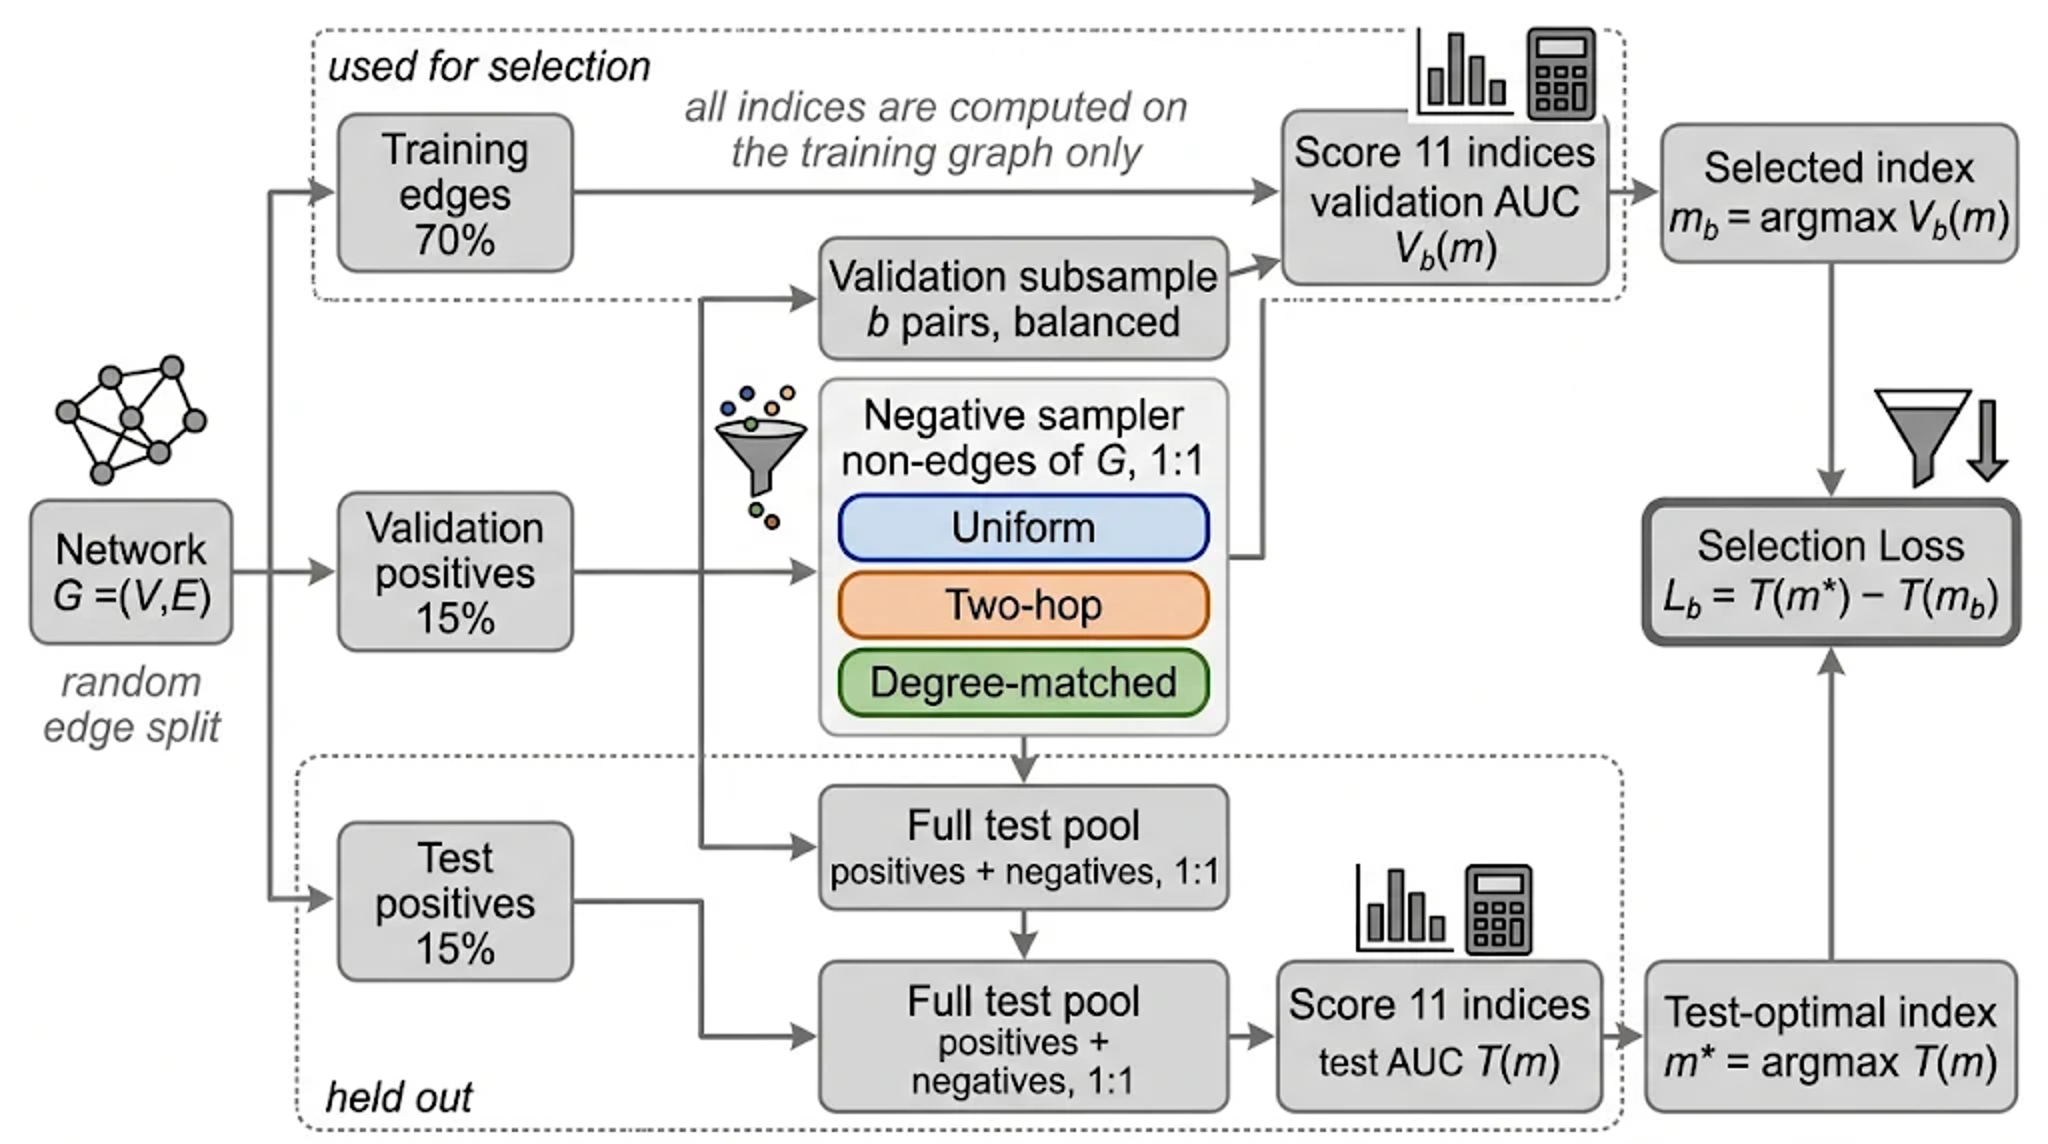
\includegraphics[width=\linewidth]{figS_protocol}
\caption{The budgeted-selection protocol. A network is split at random into 70\% training edges, 15\% validation positives and 15\% test positives. The validation pool is a balanced set of $b$ pairs, comprising $b/2$ validation positives plus $b/2$ non-edges of $G$ produced by one of three negative samplers (uniform, two-hop, degree-matched), and the eleven indices are scored on that pool by the graph built from the training edges only; the highest validation AUC is selected, $m_b=\operatorname*{arg\,max}_m V_b(m)$. The held-out block assembles the full test pool of $15\%$ test positives plus an equal number of negatives, and scores the same indices on it, which defines the test-optimal index $m^\star=\operatorname*{arg\,max}_m T(m)$. The selection loss $L_b=T(m^\star)-T(m_b)$ is the vertical distance between the two, and all of the paper's questions are questions about how it depends on $b$ and on which sampler is used on each side.}
\label{fig:protocol}
\end{figure}

Two reference quantities make the budget effect interpretable. The first is the loss obtained when the \emph{entire} validation pool is used, $L_{\mathrm{full}}$, which is the best that validation data of this kind can achieve; we call it the full-pool selection loss, and Section~\ref{sec:irreducible} shows that it is a floor in the amount of evidence rather than in its kind. The second is the requested budget actually delivered. Small networks cannot supply 2{,}000 balanced pairs, so each experiment records the effective budget $\hat b\le b$ and the fraction $\hat b/b_{\max}$ of the pool used. Budgets are $\{20,50,100,200,500,1{,}000,2{,}000\}$ pairs, and the largest requested budget exceeds the available pool on the smallest networks, which is why the effective-budget curve saturates (Figure~\ref{fig:saturation}). At the largest budget the mean effective budget across the benchmark is 1{,}284 balanced pairs, so the full-pool reference and the largest budget condition are close but not identical.

Each index is scored once on the full validation and test pools and the scores are cached; the seven budget conditions then reuse them, so the protocol costs essentially one scoring pass per repetition. AUC is the primary metric and average precision is recomputed at every budget as a secondary check.

\subsection{Design and statistical analysis}
\label{sec:stats}

The full design is 23 networks $\times$ 20 repetitions $\times$ 3 regimes $\times$ 7 budgets $=$ 9{,}660 selection experiments; each repetition uses a fresh edge split, indexed by a seed derived from the network name and the repetition number. The protocol, the budgets and the regimes were frozen before the final run and were not tuned on the results.

Uncertainty is computed at the level of networks, not repetitions: whole networks are resampled with replacement (2{,}000 bootstrap replicates for the pooled means and rates, 1{,}000 for the decay fit reported in Table~\ref{tab:decay}) and the mean loss or mis-selection rate is recomputed, giving 95\% cluster-bootstrap intervals. This is deliberately conservative, because repetitions of the same network are not independent evidence about how the method behaves across networks. Paired comparisons between regimes use the Wilcoxon signed-rank test over the 23 network-level means \citep{demsar2006statistical}. The decay model $L(b)=L_\infty+a\,b^{-\gamma}$ is fitted by bounded non-linear least squares to the per-budget means, with network-cluster bootstrap intervals for $\gamma$ (1{,}000 resamples of whole networks, re-fitting the curve at every draw). Structural correlates are Spearman correlations at a fixed budget of 100 pairs, supplemented by partial Spearman correlations that control for $\log n$, because network size is correlated with almost every other descriptor. All correlations are reported with intervals and treated as exploratory: with 23 networks the study is powered to detect large associations only.

The implementation is deliberately simple and inspectable: the eleven indices are evaluated with pre-computed neighbour sets, the negative samplers draw candidates in vectorised batches, and every reported number is produced by a single analysis script from the raw result table, so that no figure or table in the paper is transcribed by hand.

\subsection{Supplementary experiments}
\label{sec:supp}

Twelve further experiments, all on the same splits and seeds as the main run, separate the mechanisms that the budget sweep alone cannot identify. They use the twenty-three networks that can supply a balanced budget of at least eight positive pairs at the smallest budget; the twenty-edge Florentine network cannot, and is analysed separately in Appendix~\ref{app:all24}.

\emph{Noise calibration.} For every cell we draw five independent balanced validation samples at each of four budgets and record the AUC of all eleven indices on each draw. The dispersion of these draws gives the validation-noise scale $\sigma(b)$ directly, without a distributional assumption, and the covariance of the deviations across indices gives the correlation $\rho$ of the estimation errors, which matters because selection compares differences of AUCs measured on the same pairs.

\emph{Crossed regimes.} For every cell we construct validation pools under all three negative regimes and test pools under all three, and evaluate selection for each of the nine combinations at four budgets. The diagonal is the matched design of the main experiment; the six off-diagonal cells price a mismatch between the distribution used to validate and the distribution used to test.

\emph{Selection rules.} At a fixed budget $b$, one draw of $b$ pairs is compared with rules that spend the same $b$ pairs differently: eight disjoint draws of $b/8$ pairs averaged by AUC, the same draws aggregated by rank, a lower confidence bound (mean minus $\lambda$ standard deviations, $\lambda\in\{1,2\}$), a tolerance zone that keeps every candidate within one standard error of the best and then prefers the most stable one, and an empirical-Bayes (James--Stein) shrinkage of each method mean towards the candidate-set mean. Five independent single-draw baselines are averaged to reduce the Monte Carlo error of the comparison.

\emph{Hedged validation.} The same draws are repeated under each of the three regimes, and the candidate is chosen by the mean AUC across all of them. This uses the shared positive set and extra negative sampling only, so it costs no additional labelled edges.

\emph{Racing and candidate composition.} Sequential selection is implemented as successive halving at stages $b/8,b/4,b/2,b$, with an elimination margin of $c\,\sigma(b)\sqrt{2(1-\rho)}$ on the scale of an AUC difference; the constant $c$ is swept over $\{0.5,1,2,3\}$ rather than tuned, so that no configuration is favoured. Candidate composition is varied by adding a truncated Katz score, $\beta A^2+\beta^2A^3$ with $\beta=0.05$ evaluated pair by pair so that $A^3$ is never formed, and a gradient-boosted stacker over the eleven index scores trained with three-fold cross-fitting \emph{only on the same $b$ validation pairs it competes for}, so that every candidate in a comparison sees the same annotation budget.

\emph{Held-out networks.} Six SNAP networks that never entered the benchmark, the protocol or any tuning decision are run through the same budget grid with ten repetitions. They are larger and sparser than the benchmark median, and their candidate sets have far fewer near-ties, so the experiment tests where the floor of the main results should and should not appear (Section~\ref{sec:external}).

\emph{Test-pool scaling.} Eight networks are scored once on a 4{,}000-pair test pool and then evaluated on random sub-pools of 50, 100, 200, 500, 1{,}000 and 2{,}000 pairs, ten sub-pools and ten repetitions per cell, with the full-pool winner as the reference. The reported loss splits exactly into a test-resolution term and a validation term, so the experiment measures how much of the loss is the test sample's own noise (Section~\ref{sec:testpool}).

\emph{Leave-one-out hedging.} The hedged rule is evaluated twice: once averaging all three validation regimes, and once averaging only the two regimes that are not the deployment one. The second is the design a study without deployment knowledge can implement, and it is the basis of the correction in Section~\ref{sec:rules} (Table~\ref{tab:hedge}).

\emph{Temporal split.} Three timestamped SNAP networks (email-Eu-core-temporal and the two Bitcoin-OTC trust networks) are split by edge time rather than at random: the oldest 70\% of edges train, the next 15\% validate and the newest 15\% test. Edges whose endpoints never appear in the training slice are dropped and counted, so the experiment measures warm-start prediction under a genuine distribution shift (Section~\ref{sec:temporal}).

\section{A near-tie theory of selection loss}
\label{sec:theory}

A simple theory makes a testable prediction about the shape of the curves. Suppose that in a cell the true test AUCs of the candidates are $T_1,\dots,T_K$ and that the validation estimate of candidate $k$ is $\hat T_k = T_k + \varepsilon_k$ with $\varepsilon$ zero-mean, of scale $s=s(b)$ per candidate and with cross-candidate correlation $\rho$. A wrong selection happens when the noise overcomes the true gap $\Delta$ between the best and the runner-up. The expected loss conditional on that gap is $\Delta$ times the probability that the runner-up overtakes the leader, which for Gaussian noise is $\Phi(-\Delta/(s\sqrt{2(1-\rho)}))$. Averaging over cells,
\begin{equation}
\mathbb{E}[L] \;=\; \int_0^{\infty} \Delta\,\Phi\!\left(-\frac{\Delta}{s\sqrt{2(1-\rho)}}\right) g(\Delta)\,\mathrm{d}\Delta ,
\label{eq:el}
\end{equation}
where $g$ is the density of the top-two gap. If that density behaves as a power law near zero, $g(\Delta)\propto\Delta^{\alpha-1}$, substituting $\Delta=su$ gives
\begin{equation}
\mathbb{E}[L] \;\propto\; s^{1+\alpha} \;\propto\; b^{-\beta(1+\alpha)},
\qquad\text{so}\qquad \gamma=\beta(1+\alpha).
\label{eq:gamma}
\end{equation}
The step from the second to the third expression is the only modelling assumption, and it is the one earlier statements of this argument get wrong: they assume $s\propto b^{-1/2}$, the rate for an estimate from $b$ independent pairs. If the two sides of the validation pool are both finite, and if the same positives are reused across candidates, the rate is steeper; the noise calibration of Section~\ref{sec:irreducible} measures $\beta=0.55$--$0.62$. The exponent $\alpha$ can be estimated from the full-pool test AUCs, without any budget information, as the slope of $\log F(\Delta)$ against $\log\Delta$ below a cutoff, where $F$ is the empirical distribution of top-two gaps over cells. On the twenty-three networks this gives $\alpha=0.26$ (uniform), $0.34$ (two-hop) and $0.28$ (degree-matched) at a cutoff of 0.02, and $\beta(1+\alpha)=0.78$, $0.74$ and $0.79$. The intervals are wide ($0.74$--$0.92$ for the first) because $\alpha$ is estimated from a few hundred gaps, but the ordering is stable across cutoffs from 0.005 to 0.04.

The same statistic explains the heterogeneity across networks. The median top-two test gap ranges from 0.0001 AUC on CaHepTh and the Watts--Strogatz graphs, through 0.009 on ER-500, to 0.05--0.11 on the Barab\'asi--Albert graphs, and $\alpha$ estimated per network tracks that ordering. Networks with a well-separated winner have a large $\alpha$, hence a steep predicted decay and a small floor; networks with several near-tied candidates have a shallow $\alpha$ and a floor that additional labels do not remove.

Equation~\eqref{eq:gamma} predicts the decay of the noise-driven part of the loss, not of the observed curve, which also contains a floor. The two predictions are compared in Section~\ref{sec:irreducible}: the noise-only simulation, which uses the empirical gap distribution instead of the power-law tail, decays at 0.64--0.69, and the closed form at 0.74--0.79, while the fitted composite exponents are 1.11--1.42. The observed curve is steeper than its noise component because a floor makes a three-parameter power law bend, and that is why we treat \eqref{eq:decay} as a summary rather than as an estimate of a structural constant.

\section{Results}
\label{sec:results}

\subsection{Selection loss decays as a power law}
\label{sec:decay}

Table~\ref{tab:pooled} and Figure~\ref{fig:loss}(a) give the pooled loss as a function of the requested budget. Under uniform negatives the mean loss falls from 0.0156 [0.0107, 0.0213] at 20 pairs to 0.0034 [0.0011, 0.0064] at 2{,}000 pairs; under two-hop negatives from 0.0209 [0.0141, 0.0274] to 0.0021 [0.0006, 0.0047]; and under degree-matched negatives from 0.0176 [0.0130, 0.0223] to 0.0034 [0.0011, 0.0065]. Most of the reduction is achieved early: by 200 pairs the loss has already fallen by 90--92\% of its total decrease, and beyond 500 pairs the curves are flat to within 0.001 AUC.

The distribution behind those means is extremely skewed, and this matters for how the numbers should be read. The median loss is 0.0007 or less at 20 pairs and exactly zero from 100 pairs onward, and at 2{,}000 pairs 68.6\% of cells are exactly right: the selected index is the test-optimal one. The mean is therefore a tail, not a level shared by all cells. That tail is concentrated at the network level too: nine of the twenty-three networks have exactly zero mean loss at 2{,}000 pairs under every regime, and three small near-tied graphs account for most of the pooled mean: Karate (0.017), Les Mis\'erables (0.013) and the sparse ER-500 graph (0.013). The other networks contribute between 0 and 0.006. Including Florentine, the twenty-edge network excluded from the main analysis, raises the pooled mean by a factor of 1.2--1.4 at the smallest budgets and by about three at 500 pairs and beyond, without changing the fitted exponent at all (Appendix~\ref{app:all24} reports the comparison), which is a warning about pooled means on heterogeneous benchmark suites.

The shape is captured by \eqref{eq:decay} with $R^2>0.99$ in all three regimes (Table~\ref{tab:decay}):
\begin{equation}
L(b) \;=\; L_\infty + a\,b^{-\gamma},
\label{eq:decay}
\end{equation}
with $\gamma=1.11$ [0.59, 1.61] for uniform, $1.33$ [0.55, 1.52] for two-hop and $1.42$ [0.48, 1.82] for degree-matched negatives. A budget increase by a factor of ten therefore reduces the budget-dependent part of the loss by roughly a factor of thirteen at $\gamma=1.11$; equivalently, doubling the budget removes 54--64\% of what remains. The exponents are estimated from seven points and their intervals are wide, which is itself a sign that a three-parameter fit to a curve with a floor is only weakly identified. We therefore report \eqref{eq:decay} as an accurate summary of the shape, and Section~\ref{sec:irreducible} asks what the composite exponent is actually made of.

\begin{table}[htbp]
\centering
\scriptsize
\setlength{\tabcolsep}{4pt}
\caption{Pooled selection loss and mis-selection rate by negative-sampling regime and requested validation budget, on the twenty-three networks that support the full protocol.}
\label{tab:pooled}
\begin{tabular}{l r l r r r r}
\toprule
Regime & Budget & Mean loss [95\% CI] & Median loss & Mis-selection (\%) & Selected AUC & Oracle AUC \\
\midrule
Uniform non-edges & 20 & 0.0156 [0.0107, 0.0213] & 0.0007 & 67.8 & 0.720 & 0.736 \\
 & 50 & 0.0079 [0.0052, 0.0112] & 0.0002 & 59.3 & 0.728 & 0.736 \\
 & 100 & 0.0049 [0.0029, 0.0075] & 0.0002 & 58.0 & 0.731 & 0.736 \\
 & 200 & 0.0043 [0.0020, 0.0070] & 0.0001 & 54.6 & 0.731 & 0.736 \\
 & 500 & 0.0035 [0.0013, 0.0065] & 0.0000 & 48.3 & 0.732 & 0.736 \\
 & 1000 & 0.0033 [0.0011, 0.0063] & 0.0000 & 47.2 & 0.732 & 0.736 \\
 & 2000 & 0.0034 [0.0011, 0.0064] & 0.0000 & 44.3 & 0.732 & 0.736 \\
\addlinespace[2pt]
Two-hop non-edges & 20 & 0.0209 [0.0141, 0.0274] & 0.0000 & 47.4 & 0.556 & 0.577 \\
 & 50 & 0.0073 [0.0043, 0.0108] & 0.0000 & 35.9 & 0.570 & 0.577 \\
 & 100 & 0.0050 [0.0028, 0.0078] & 0.0000 & 37.4 & 0.572 & 0.577 \\
 & 200 & 0.0040 [0.0021, 0.0065] & 0.0000 & 33.0 & 0.573 & 0.577 \\
 & 500 & 0.0026 [0.0009, 0.0050] & 0.0000 & 27.4 & 0.574 & 0.577 \\
 & 1000 & 0.0023 [0.0007, 0.0047] & 0.0000 & 26.1 & 0.575 & 0.577 \\
 & 2000 & 0.0021 [0.0006, 0.0047] & 0.0000 & 26.5 & 0.575 & 0.577 \\
\addlinespace[2pt]
Degree-matched non-edges & 20 & 0.0176 [0.0130, 0.0223] & 0.0009 & 59.6 & 0.726 & 0.743 \\
 & 50 & 0.0073 [0.0045, 0.0103] & 0.0000 & 50.2 & 0.736 & 0.743 \\
 & 100 & 0.0048 [0.0025, 0.0076] & 0.0000 & 43.9 & 0.739 & 0.743 \\
 & 200 & 0.0045 [0.0021, 0.0074] & 0.0000 & 40.0 & 0.739 & 0.743 \\
 & 500 & 0.0035 [0.0011, 0.0065] & 0.0000 & 34.6 & 0.740 & 0.743 \\
 & 1000 & 0.0035 [0.0010, 0.0065] & 0.0000 & 29.1 & 0.740 & 0.743 \\
 & 2000 & 0.0034 [0.0011, 0.0065] & 0.0000 & 26.5 & 0.740 & 0.743 \\
\addlinespace[2pt]
\bottomrule
\end{tabular}
\par\vspace{2pt}\begin{minipage}{\linewidth}\footnotesize Selection loss is the test-AUC gap between the validation-selected index and the test-optimal index, averaged over networks, repetitions and budgets. Brackets give 95\% bootstrap intervals resampling networks (B = 2{,}000). The median is reported next to the mean because the loss distribution is heavy-tailed; the budget is the requested number of balanced validation pairs, on 23 networks.\end{minipage}
\end{table}

\begin{table}[htbp]
\centering
\scriptsize
\caption{Fitted decay of the mean selection loss on twenty-three networks.}
\label{tab:decay}
\begin{tabular}{l r r l r}
\toprule
Regime & $L_\infty$ & $a$ & $\gamma$ [95\% CI] & $R^2$ \\
\midrule
Uniform non-edges & 0.0032 & 0.3442 & 1.11 [0.59, 1.61] & 0.998 \\
Two-hop non-edges & 0.0024 & 0.9880 & 1.33 [0.55, 1.52] & 0.996 \\
Degree-matched non-edges & 0.0035 & 0.9899 & 1.42 [0.48, 1.82] & 0.998 \\
\bottomrule
\end{tabular}
\par\vspace{2pt}\begin{minipage}{\linewidth}\footnotesize Fit of $L(b) = L_\infty + a\,b^{-\gamma}$ to the mean selection loss at 23 networks, 7 budgets and all repetitions; the interval is a network-cluster bootstrap over 1{,}000 resamples. The three parameters are weakly identified individually --- a lower asymptote and a slower decay fit the same curve almost as well --- so the fit is descriptive and the closed form of Section~\ref{sec:theory} is what identifies $\gamma$.\end{minipage}
\end{table}

\begin{figure}[htbp]
\centering
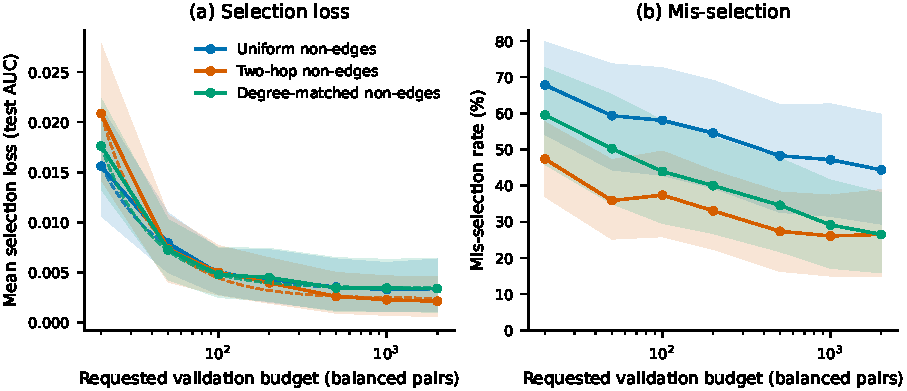
\includegraphics[width=\linewidth]{fig1_loss_and_misselection}
\caption{Selection loss (a) and mis-selection rate (b) against the requested validation budget, by negative-sampling regime. Points are means over 23 networks and 20 repetitions; shaded bands are 95\% network-level cluster-bootstrap intervals (2{,}000 resamples of whole networks); dashed curves are the fitted power laws of \eqref{eq:decay}.}
\label{fig:loss}
\end{figure}

Figure~\ref{fig:saturation} shows why the two rightmost budget conditions are nearly redundant on small networks: the requested budget exceeds the available validation pool, so the effective budget saturates. On average, a request of 2{,}000 pairs is realised as 1{,}284 pairs, and on the smallest networks as fewer than 300. This is the mechanism that produces the apparent plateau in earlier pilot work; the fitted curve of \eqref{eq:decay} uses the effective rather than the requested budget, so the plateau is not an artefact of the fit.

\begin{figure}[htbp]
\centering
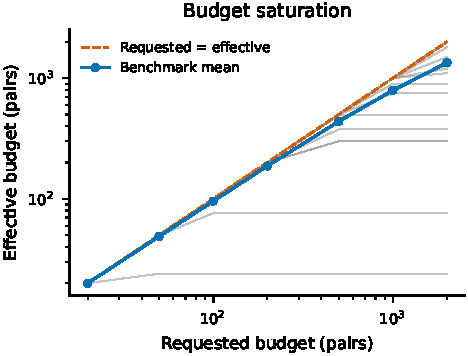
\includegraphics[width=0.70\linewidth]{figS_saturation}
\caption{Requested versus effective validation budget. Grey lines are the 23 individual networks; the blue line is the benchmark mean over those networks and 20 repetitions; the dashed line marks perfect delivery. Small networks cannot supply the largest requested budgets.}
\label{fig:saturation}
\end{figure}

\subsection{The plateau is not sampling noise}
\label{sec:irreducible}

The most informative part of the curve is not the exponent but the plateau. If selection loss were purely a finite-sample phenomenon, more validation data would drive it to zero. It does not: selecting on the complete validation pool leaves a mean loss of 0.0033 [0.0010, 0.0061] under uniform negatives, 0.0020 [0.0005, 0.0045] under two-hop negatives and 0.0032 [0.0009, 0.0063] under degree-matched negatives, which agree with the fitted asymptotes $L_\infty$ (0.0032, 0.0024 and 0.0035) to within 0.0004 AUC in every regime. Figure~\ref{fig:decomp} shows the two components separately.

\begin{figure}[htbp]
\centering
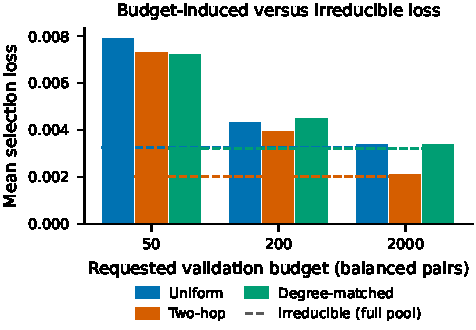
\includegraphics[width=0.78\linewidth]{fig5_decomposition}
\caption{Budget-induced versus full-pool selection loss at three budgets, by negative-sampling regime. Bars are the mean loss at each budget over 23 networks and 20 repetitions; dashed segments mark the loss obtained with the full validation pool on the same networks. By 2{,}000 pairs the bars have reached the full-pool level.}
\label{fig:decomp}
\end{figure}

The natural reading of such a plateau is that it is the sampling noise of an AUC estimate that cannot be reduced without more labels. That reading is testable, and it is wrong. The variance of an AUC estimate, and of a difference between two AUCs measured on correlated samples, is classical \citep{hanley1982meaning,delong1988comparing}. The noise calibration experiment measures both quantities directly. The standard deviation of a validation AUC at 100 pairs is $\sigma(100)=0.029$ under uniform negatives, $0.035$ under two-hop and $0.030$ under degree-matched negatives, and it scales as $b^{-\beta}$ with $\beta=0.62$, $0.55$ and $0.61$ respectively---steeper than the $b^{-1/2}$ of an independent-sample argument, because the positive and the negative side of a balanced pool are both finite and the same positives are reused across indices. The estimation errors of different indices are strongly correlated, $\rho=0.73$ for uniform and degree-matched negatives and $\rho=0.49$ for two-hop negatives, because the indices are scored on the same pairs; a comparison of two indices therefore has noise $\sigma(b)\sqrt{2(1-\rho)}$, roughly two thirds of the naive value.

Feeding these measured quantities, together with the observed test-AUC vector of each cell, into a noise-only simulation answers the question directly: how much loss would selection incur if validation noise were the only mechanism? Table~\ref{tab:floor} gives the answer, and Figure~\ref{fig:floor} shows the two components separately. At 2{,}000 pairs the noise model predicts 0.0002--0.0005 AUC against an observed 0.0021--0.0034, i.e.\ between 7\% and 22\% of the plateau. At the smallest budget it accounts for a quarter to a half of the loss (50\% under two-hop negatives, where the noise scale is largest). The plateau is therefore not sampling error, but neither is it a level that every study pays. Because the top-two gap has a heavy lower tail, the loss distribution is a mixture: its median is zero, 68.6\% of selections are exactly optimal, and the mean plateau is the average over a minority of near-tied cells whose ranking flips between two realizations of the same distribution. Those flips are not removed by adding further pairs of the same kind, because the two pools are different samples of non-edges rather than one growing sample; they are removed by changing what the candidates are compared against, which is the subject of Section~\ref{sec:shift}.

\begin{table}[htbp]
\centering
\footnotesize
\caption{Decomposition of the observed selection loss into a validation-noise component, simulated from the \emph{measured} noise scale $\sigma(b)$ and the observed gap structure, and a residual that the model does not explain. The lower block compares three decay exponents.}
\label{tab:floor}
\begin{tabular}{l r r r r r}
\toprule
Regime & Budget & $\sigma(b)$ & Observed & Noise model & Residual \\
\midrule
Uniform & 20 & 0.0616 & 0.0156 & 0.0045 & +0.0111 \\
Uniform & 200 & 0.0148 & 0.0043 & 0.0010 & +0.0033 \\
Uniform & 2000 & 0.0035 & 0.0034 & 0.0002 & +0.0032 \\
\addlinespace[3pt]
Two-hop & 20 & 0.0675 & 0.0209 & 0.0105 & +0.0104 \\
Two-hop & 200 & 0.0189 & 0.0040 & 0.0023 & +0.0017 \\
Two-hop & 2000 & 0.0053 & 0.0021 & 0.0005 & +0.0017 \\
\addlinespace[3pt]
Degree-matched & 20 & 0.0645 & 0.0176 & 0.0058 & +0.0119 \\
Degree-matched & 200 & 0.0158 & 0.0045 & 0.0012 & +0.0033 \\
Degree-matched & 2000 & 0.0038 & 0.0034 & 0.0003 & +0.0031 \\
\addlinespace[3pt]
\midrule
Regime & $\gamma$ fitted & $\gamma$ noise model & $\gamma=\beta(1+\alpha)$ & Share noise at $b=2000$ & Residual at $b=2000$ \\
\midrule
Uniform & 1.11 & 0.64 & 0.78 & 7\% & +0.0032 \\
Two-hop & 1.33 & 0.69 & 0.74 & 22\% & +0.0017 \\
Degree-matched & 1.42 & 0.69 & 0.79 & 10\% & +0.0031 \\
\bottomrule
\end{tabular}
\par\vspace{2pt}\begin{minipage}{\linewidth}\footnotesize $\sigma(b)$ is the measured standard deviation of a validation AUC at budget $b$, averaged over methods and cells. The noise model draws validation AUCs with this scale around the true test AUC, using the \emph{measured} cross-method correlation ($\rho=0.48$--$0.73$) and $500$ draws per cell. Residual is the part of the observed loss that the noise model does not explain; it contains the test pool's own resolution, the saturation of small pools, and any structural disagreement between the validation and test samples, and should not be read as a pure distribution-shift term (Section~\ref{sec:shift} measures that separately). The closed form is $\gamma=\beta(1+\alpha)$ with $\beta$ measured from the noise calibration and $\alpha$ from the full-pool gaps.\end{minipage}
\end{table}

\begin{figure}[htbp]
\centering
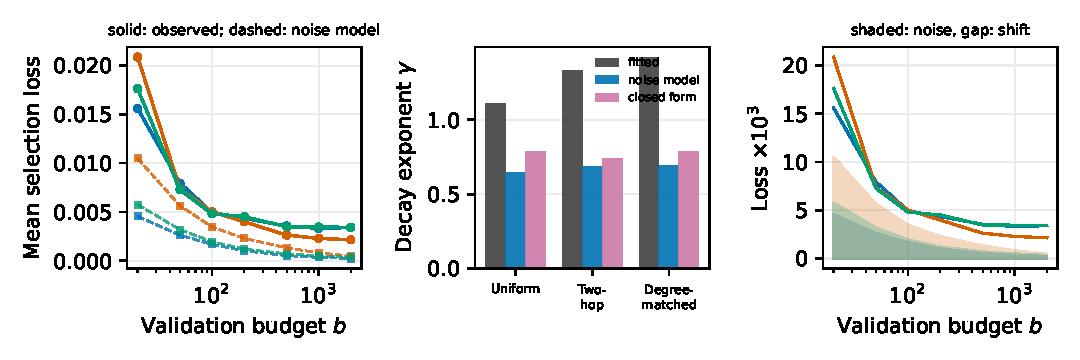
\includegraphics[width=\linewidth]{fig7_theory}
\caption{Decomposition of the selection-loss curve. (a) Observed loss (solid) and the loss produced by validation noise alone (dashed), simulated with the measured noise scale and cross-method correlation. (b) Decay exponents: fitted to the observations, implied by the noise model, and predicted by the near-tie closed form $\gamma=\beta(1+\alpha)$ with the measured $\beta$. (c) Stacked view for the uniform regime: the shaded area is the part of the simulated loss attributable to validation noise, the gap to the solid line is the residual. Shaded bands in (a) and (c) are 95\% network-cluster bootstrap intervals over the 23 networks; points are means over those networks and 20 repetitions.}
\label{fig:floor}
\end{figure}

The same measurement reconciles the theory with the fitted curve, and shows why the fitted exponent should not be read structurally. The closed form of Section~\ref{sec:theory} predicts $\gamma=\beta(1+\alpha)=0.74$--$0.79$ from the measured noise decay and the measured near-tie density, and the noise model, which uses the empirical gap distribution rather than the closed form, independently produces 0.64--0.69. The two agree in the sense that matters: a noise-only mechanism decays at roughly two thirds, not at 1.1--1.4. The exponent fitted to the observations is larger precisely because the observations are the sum of a decaying term and a floor, and a three-parameter power law fitted to such a curve is only weakly identified---its intervals span 0.48--1.82. We therefore report \eqref{eq:decay} as an accurate three-parameter summary of the curve, but not as an estimate of a fundamental exponent. The mechanism-level statement is the one supported by the decomposition: the budget-dependent part decays with an exponent of about two thirds, as the near-tie argument with the measured noise decay predicts, and the floor is not noise.

\subsection{The test pool's own resolution is not the floor}
\label{sec:testpool}

A second candidate explanation for the residual is the test set itself. Every number above is measured against the best index \emph{on the same test pool}, so if that pool is small the winner is defined noisily and part of the apparent loss may be the test sample's resolution rather than the selection procedure's. The experiment of Table~\ref{tab:testpool} separates the two. Eight networks are scored once on a 4{,}000-pair test pool, then evaluated on sub-pools of 50 to 2{,}000 pairs against the full-pool winner. The reported loss splits exactly into a \emph{test-resolution} term (the gap between the best index on the sub-pool and the best on the full pool) and a \emph{validation} term (the gap between the full-pool winner and the index the budget selected).

\begin{table}[htbp]
\centering
\scriptsize
\caption{Where the floor comes from: the reported loss at the largest validation budget (2{,}000 pairs) split into the cost of defining the winner on a finite test pool and the cost of choosing it with a finite validation pool. Eight networks, ten repetitions, uniform negatives.}
\label{tab:testpool}
\begin{tabular}{r r r r r}
\toprule
Test pool (pairs) & Test-resolution term & Validation term & Total loss & Test-AUC s.d. \\
\midrule
50 & 0.0022 & -0.0000 & 0.0021 & 0.0285 \\
100 & 0.0011 & 0.0002 & 0.0012 & 0.0203 \\
200 & 0.0005 & 0.0001 & 0.0006 & 0.0139 \\
500 & 0.0001 & 0.0002 & 0.0003 & 0.0081 \\
1000 & 0.0000 & 0.0001 & 0.0001 & 0.0052 \\
2000 & 0.0000 & 0.0001 & 0.0001 & 0.0025 \\
\bottomrule
\end{tabular}
\par\vspace{2pt}\begin{minipage}{\linewidth}\footnotesize The two terms are measured on the same test sub-pool and sum exactly to the total. The test-resolution term is the gap between the best index on the sub-pool and the best on the full 4{,}000-pair pool; the validation term is the gap between the full-pool winner and the index selected with the validation budget. Test-AUC s.d. is the standard deviation of a single index's AUC across sub-pools of that size.\end{minipage}
\end{table}

\begin{figure}[htbp]
\centering
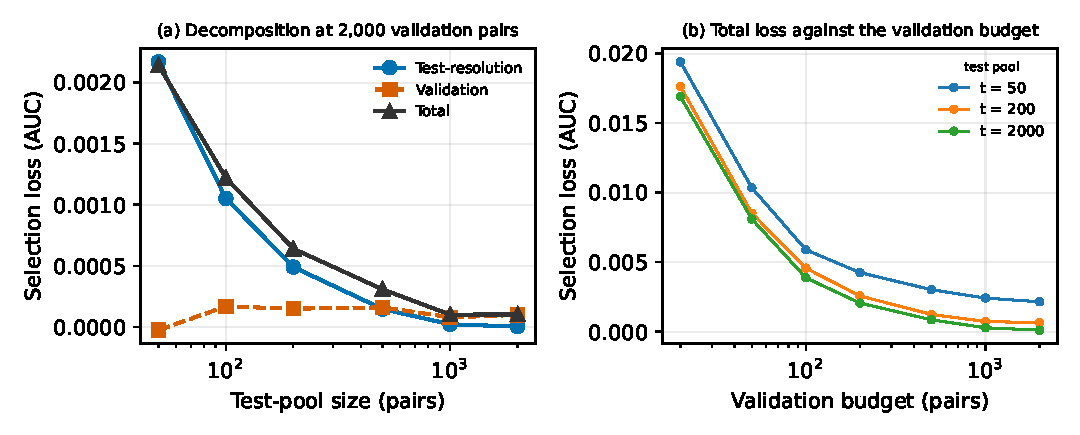
\includegraphics[width=\linewidth]{fig15_test_pool}
\caption{Test-pool scaling. (a) At 2{,}000 validation pairs the loss splits into a test-resolution term and a validation term; the former is 0.0022 AUC at a 50-pair test pool and vanishes beyond 500 pairs. (b) Total loss against the validation budget for three test-pool sizes.}
\label{fig:testpool}
\end{figure}

Test resolution is real but small: 0.0022 AUC at a 50-pair test pool, 0.0001 at 500 pairs and below $10^{-4}$ from 1{,}000 pairs, while the validation term at 2{,}000 pairs is $9.9\times10^{-5}$ on these networks. The standard deviation of a single index's AUC across sub-pools scales as $t^{-0.64}$, the same exponent as the validation noise, which is a useful consistency check: the two noises are the same estimator applied to pools of different size. Two conclusions follow. First, the residual floor of Section~\ref{sec:irreducible} is not a test-pool artefact: on the eight large networks studied here the total loss at 2{,}000 validation pairs is 0.0001--0.0008, an order of magnitude below the pooled mean, because these networks are large and their candidate sets are not near-tied. Second, studies that report test AUC on pools of a few dozen pairs per class cannot resolve differences below about 0.002 AUC at all, which is the same order as the selection losses this paper is about. Reporting the test-pool size is therefore as important as reporting the validation budget.

\subsection{A forecast from measured noise, tested against observation}
\label{sec:forecast}

The decomposition above is descriptive: it attributes what validation noise cannot explain to shift. A stronger test is to predict the joint effect from measured quantities and compare with observation. We simulate selection with validation noise of scale $\sigma(b)=\sigma(100)(b/100)^{-\beta}$ ($\beta$ measured per regime), and evaluate the reported loss on a test pool whose noise has scale $\sigma_{\text{test}}(t)$ and the \emph{measured} $11\times11$ cross-index correlation matrix of test sub-pools. The population AUC vector is the full-pool vector of the test-pool experiment, and the gap distribution is the empirical one: no parametric tail is assumed.

\begin{figure}[htbp]
\centering
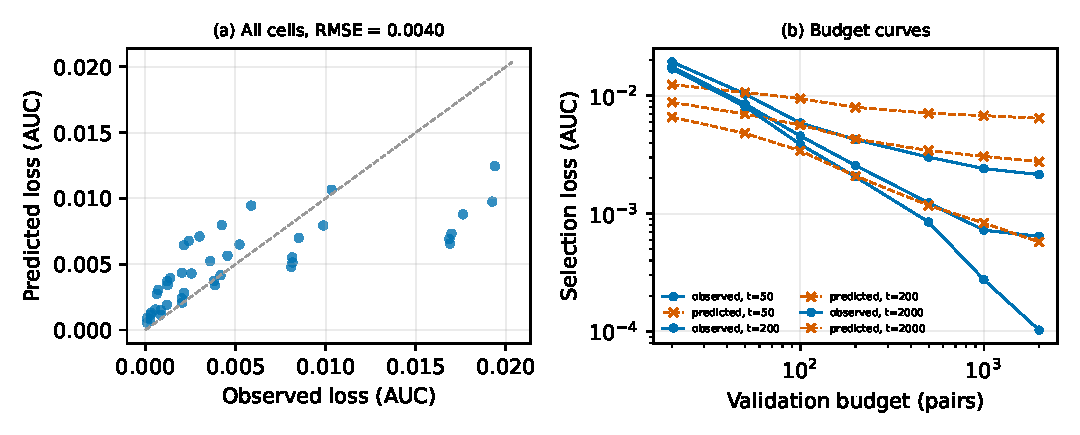
\includegraphics[width=\linewidth]{fig16_forecast}
\caption{Two-noise forecast against observation. (a) Predicted versus observed loss for every (budget, test size) cell of the test-pool experiment; the diagonal is perfect prediction. (b) Observed (solid) and predicted (dashed) budget curves at three test-pool sizes.}
\label{fig:forecast}
\end{figure}

The forecast reproduces the level of the loss accurately at large test pools, giving 0.0021 predicted against 0.0021 observed at 200 validation pairs and a 2{,}000-pair test pool, and over-predicts at very small ones (0.0080 against 0.0042 at a 50-pair pool), because the nine common-neighbour indices are near-duplicates whose test AUCs move together even more tightly than the averaged correlation matrix allows. Across all 42 cells the correlation between prediction and observation is 0.78 and the root-mean-square error is 0.0040 AUC. The forecast gets the level right but not the curvature: it predicts a log--log slope of $-0.55$ where the observed curves are steeper ($-1.10$). We do not attribute the difference to a structural term, because a floor added to a decaying curve lowers the slope rather than raising it; the curvature difference is instead consistent with the forecast's under-statement of the coupling among the near-duplicate indices at small validation budgets, and we leave it open. What the exercise establishes is that the two measured noise sources plus the empirical gap distribution are enough to account for the loss at large budgets, so the residual in Table~\ref{tab:floor} is a residual component rather than a modelling artefact.

\subsection{The price of a validation/deployment mismatch}
\label{sec:shift}

If the plateau is not noise, it must come from the validation and test evidence differing in a way that more data of the same kind cannot fix. The crossed-regime experiment measures that difference directly, by validating under one negative-sampling regime and testing under another. Table~\ref{tab:shift} and Figure~\ref{fig:shift} give the $3\times3$ matrix at a budget of 200 pairs.

\begin{table}[htbp]
\centering
\scriptsize
\setlength{\tabcolsep}{4pt}
\caption{Cost of a validation/deployment mismatch at a budget of 200 pairs. Rows are the negative-sampling regime used to validate, columns the regime used to test. The diagonal is the matched design. The two bottom rows summarise the hedged rule (validate on all three regimes, average the AUCs) and the matched reference on the same scale.}
\label{tab:shift}
\begin{tabular}{l r r r}
\toprule
Validation regime & Uniform & Two-hop & Degree-matched \\
\midrule
Uniform & 0.0043 & 0.0776 & 0.0095 \\
Two-hop & 0.0213 & 0.0042 & 0.0274 \\
Degree-matched & 0.0068 & 0.1060 & 0.0045 \\
\midrule
Hedged (mean AUC) & 0.0064 & 0.0128 & 0.0087 \\
Matched (reference) & 0.0039 & 0.0041 & 0.0047 \\
\bottomrule
\end{tabular}
\par\vspace{2pt}\begin{minipage}{\linewidth}\footnotesize Mean selection loss over 23 networks, twenty repetitions, three test regimes. Florentine (20 edges) is excluded because a balanced budget cannot be formed.\end{minipage}
\end{table}

\begin{figure}[htbp]
\centering
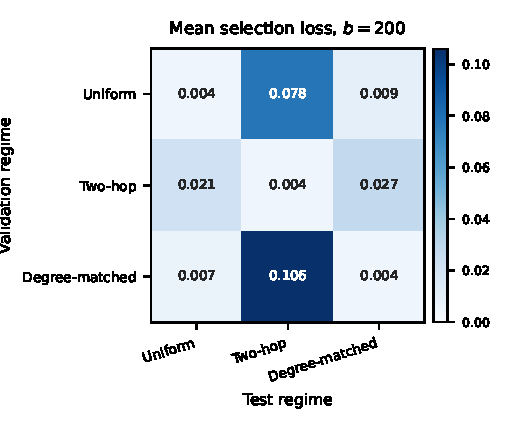
\includegraphics[width=0.70\linewidth]{fig8_shift}
\caption{Mean selection loss when the negative-sampling regime used for validation differs from the regime used for testing (200 pairs). The diagonal is the matched design. Validating on uniform negatives and testing on two-hop negatives costs eighteen times the matched loss.}
\label{fig:shift}
\end{figure}

The matrix is far from symmetric, and its largest entry is an order of magnitude above the diagonal. Validating on uniform negatives and testing on two-hop negatives costs 0.073 AUC, against 0.004 for the matched design; validating on degree-matched negatives and testing on two-hop costs 0.106; validating on two-hop and testing on uniform costs 0.021. The asymmetry has a simple reading: uniform negatives are dominated by low-degree non-edges, so a validation ranking on them rewards degree-driven scores, whereas two-hop negatives are hard cases that reward neighbourhood overlap. A study that validates on easy negatives and deploys on hard ones therefore loses more than precision: it selects the wrong family of index.

In practice this changes two things. First, the negative-sampling regime is a first-order design decision, larger in its effect than any budget choice in this paper: the 0.10 AUC difference between the best and the worst cell of the matrix dwarfs the 0.012 AUC that separates a budget of 20 pairs from a budget of 2{,}000. Reporting the regime is therefore not a detail of the protocol; it is part of the result. Second, the floor of the matched design is not a lower bound on what a mismatched study will experience. A paper that validates on uniform negatives and is later deployed against a two-hop candidate generator should expect roughly the off-diagonal entry, not the diagonal one.

\subsection{Selection rules and hedged validation}
\label{sec:rules}

The decomposition suggests two ways to attack the plateau: spend the same annotation budget more cleverly, or change what is validated against. We tested the first and it does not work; the second does.

Table~\ref{tab:rules} compares five rules that spend the same $b$ pairs as the single draw they are measured against. Averaged multi-draw validation divides the budget into eight disjoint draws and averages the AUCs; rank aggregation averages the within-draw ranks; a lower confidence bound subtracts $\lambda$ standard deviations from the mean; a tolerance zone keeps every candidate within one standard error of the leader and prefers the most stable; and empirical-Bayes shrinkage pulls each candidate towards the set mean by an amount set by its own standard error. No rule beats the single draw at any budget. Averaging is the least harmful, costing $+0.0029$ AUC at 50 pairs ($p=2\times10^{-4}$), $+0.0006$ at 200 ($p=0.008$) and $+0.0004$ at 500 (not significant). Shrinkage is second, at $+0.0037$ ($p=1\times10^{-4}$), $+0.0008$ ($p=0.006$) and $+0.0005$ (not significant) over the same budgets. Rank aggregation and the confidence bound are the worst, at $+0.030$ and $+0.028$ AUC at 50 pairs. The share of \emph{networks} on which a rule improves on the single draw stays between 0 and 35\% throughout. The $p$-values are computed over the 23 network means, not over the several hundred cells: repetitions of one network reuse its edges and are not independent observations, and treating them as such would understate every $p$-value by an order of magnitude.

\begin{table}[htbp]
\centering
\scriptsize
\setlength{\tabcolsep}{4pt}
\caption{Five selection rules at a fixed annotation budget, matched design. Every rule spends exactly the same number of pairs as the single draw it is compared with; differences are paired within network.}
\label{tab:rules}
\begin{tabular}{l r r r r}
\toprule
Rule & Mean loss & $\Delta$ vs single & $p$ (Wilcoxon) & Networks better (\%) \\
\midrule
\multicolumn{5}{l}{Budget 50 pairs} \\
\quad Single draw & 0.0088 & --- & --- & --- \\
\quad Averaged AUC & 0.0117 & +0.0029 & 0.00021 & 26 \\
\quad Rank aggregation & 0.0384 & +0.0295 & 7.9e-06 & 13 \\
\quad Tolerance zone & 0.0172 & +0.0084 & 7.9e-06 & 13 \\
\quad Lower confidence bound & 0.0367 & +0.0279 & 2.4e-07 & 0 \\
\quad Shrinkage (empirical Bayes) & 0.0126 & +0.0037 & 0.00011 & 17 \\
\addlinespace[2pt]
\multicolumn{5}{l}{Budget 100 pairs} \\
\quad Single draw & 0.0054 & --- & --- & --- \\
\quad Averaged AUC & 0.0065 & +0.0011 & 0.0039 & 22 \\
\quad Rank aggregation & 0.0170 & +0.0115 & 7.3e-05 & 13 \\
\quad Tolerance zone & 0.0112 & +0.0057 & 4.8e-07 & 4 \\
\quad Lower confidence bound & 0.0176 & +0.0122 & 2.4e-07 & 0 \\
\quad Shrinkage (empirical Bayes) & 0.0073 & +0.0019 & 0.00011 & 13 \\
\addlinespace[2pt]
\multicolumn{5}{l}{Budget 200 pairs} \\
\quad Single draw & 0.0043 & --- & --- & --- \\
\quad Averaged AUC & 0.0049 & +0.0006 & 0.008 & 17 \\
\quad Rank aggregation & 0.0082 & +0.0038 & 0.00069 & 22 \\
\quad Tolerance zone & 0.0071 & +0.0028 & 6.1e-05 & 9 \\
\quad Lower confidence bound & 0.0098 & +0.0054 & 7e-05 & 4 \\
\quad Shrinkage (empirical Bayes) & 0.0052 & +0.0008 & 0.0062 & 17 \\
\addlinespace[2pt]
\multicolumn{5}{l}{Budget 500 pairs} \\
\quad Single draw & 0.0036 & --- & --- & --- \\
\quad Averaged AUC & 0.0039 & +0.0004 & 0.21 & 35 \\
\quad Rank aggregation & 0.0043 & +0.0008 & 0.064 & 22 \\
\quad Tolerance zone & 0.0050 & +0.0014 & 0.0002 & 0 \\
\quad Lower confidence bound & 0.0053 & +0.0018 & 0.00033 & 9 \\
\quad Shrinkage (empirical Bayes) & 0.0041 & +0.0005 & 0.12 & 26 \\
\addlinespace[2pt]
\bottomrule
\end{tabular}
\par\vspace{2pt}\begin{minipage}{\linewidth}\footnotesize Mean over 23 networks and twenty repetitions, matched design. Each network contributes one mean difference (averaged over its repetitions and regimes) and $p$ is a paired Wilcoxon signed-rank test over the 23 networks, not over cells: repetitions of one network are not independent observations. A positive $\Delta$ means the rule is worse than a single draw of the same size.\end{minipage}
\end{table}

The failure is not a tuning artefact, and it has a statistical explanation. At a fixed total budget, splitting the pairs into $R$ draws and averaging cannot reduce the variance of the AUC estimate: the mean of $R$ estimates of $b/R$ pairs has variance $\sigma^2(b/R)/R$. If the noise scaled exactly as $b^{-1/2}$ this would equal $\sigma^2(b)$, so splitting would gain no information. Because the measured noise decays more slowly, as $b^{-0.55}$ to $b^{-0.62}$, the variance of the average is larger than that of a single draw by a factor $R^{2(0.60)-1}=R^{0.2}$, about 1.5 for $R=8$. Averaging is therefore not neutral but mildly harmful, which is what the measurements show. The ranking and confidence-bound rules do worse still, because they estimate a stability quantity from the same small draws that generate the noise they are trying to control, and the estimate of stability is itself the noisiest quantity in the problem. The plateau, being a near-tie effect rather than a variance effect, is untouched by all of them.

The second route does work. Because the positives of a cell are shared, the negative sampler is the only thing that changes across regimes, and negative sampling costs computation rather than annotation. Hedged validation therefore validates under all three regimes, averages the AUCs across them, and selects. Table~\ref{tab:hedge} and Figure~\ref{fig:rules}(b) compare it with the two alternatives a study actually faces: knowing the deployment regime (matched) and guessing it wrongly.

\begin{table}[htbp]
\centering
\scriptsize
\caption{Hedged validation at a budget of 200 pairs, with the deployment regime unknown. \emph{Matched} validates under the deployment regime; \emph{mismatched} is the mean of the two single wrong regimes; \emph{hedge, two regimes} averages only the two regimes that are not the deployment one; \emph{hedge, all three} also includes it. Loss is in test AUC.}
\label{tab:hedge}
\begin{tabular}{l r r r r r}
\toprule
Deployment regime & Matched & Mismatched & Hedge (two) & Hedge (three) & Recovery, two / three \\
\midrule
Uniform & 0.0039 & 0.0140 & 0.0124 & 0.0064 & 12\% / 55\% \\
Two-hop & 0.0041 & 0.0918 & 0.0878 & 0.0128 & 4\% / 86\% \\
Degree-matched & 0.0047 & 0.0184 & 0.0181 & 0.0087 & 2\% / 53\% \\
\bottomrule
\end{tabular}
\par\vspace{2pt}\begin{minipage}{\linewidth}\footnotesize The recovery is the share of the mismatch penalty removed, relative to the mean of the two single wrong regimes, at the same annotation budget: hedging spends extra negative sampling, not extra labels. The recovery is large only where the deployment regime is two-hop, because the two-hop penalty is an order of magnitude larger than the other two; hedging over the two regimes that exclude two-hop recovers little of it.\end{minipage}
\end{table}

\begin{figure}[htbp]
\centering
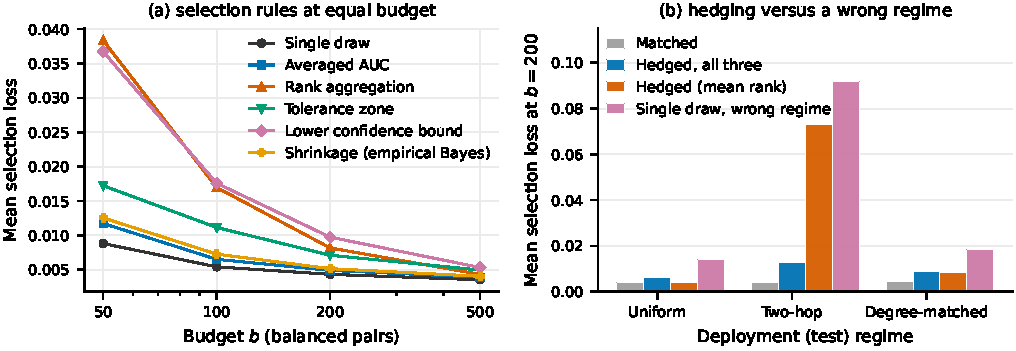
\includegraphics[width=\linewidth]{fig9_rules_hedge}
\caption{(a) Selection rules at equal annotation budget, matched design. The single draw is not beaten by any of them. (b) Hedged validation against the matched design and against a mismatched validation regime, at 200 pairs. Hedging costs a little when the regime is known and saves most of the penalty when it is not.}
\label{fig:rules}
\end{figure}

Table~\ref{tab:hedge} makes the limitation explicit, and it is the most important qualification in the paper. The 86\% recovery figure quoted above is one minus the ratio of the hedged loss to the mismatched loss, and it holds only for the two-hop column \emph{and} only when the two-hop regime is itself one of the regimes hedged: averaging all three validation AUCs includes the deployment regime, which is exactly the information a study without a deployment regime does not have. Hedging instead over the other two regimes, which is the leave-one-out design, recovers 12\% of the penalty under uniform deployment, 4\% under two-hop and 2\% under degree-matched negatives, i.e.\ almost nothing. The reason is arithmetic: the two-hop penalty is an order of magnitude larger than the other two (0.092 against 0.014 and 0.018), so a hedge that excludes two-hop cannot buy down a two-hop penalty. What hedging over all three does buy is robustness to \emph{not knowing} the deployment regime: it costs 0.0128 AUC under two-hop deployment against 0.0041 matched, but it is also the only rule whose loss stays below 0.013 in every column, whereas a single wrong regime costs up to 0.092. It is insurance costing about twice the matched loss, not a free lunch, and we report it as such.

\subsection{Sequential selection does not pay for itself}
\label{sec:racing}

If annotation is the scarce resource, an adaptive rule that stops early when one candidate is clearly ahead would be worth more than a better estimator. Such rules are standard in model selection and best-arm identification \citep{maron1994hoeffding,karnin2013almost}. Table~\ref{tab:racing} tests the standard implementation: successive halving over four stages, with elimination at a margin calibrated to the measured noise of an AUC \emph{difference} and swept over a grid of constants so that no single tuning is favoured.

\begin{table}[htbp]
\centering
\scriptsize
\setlength{\tabcolsep}{4pt}
\caption{Racing against a fixed validation budget, with the elimination margin swept over four constants $c$ on the scale of the measured noise of an AUC difference. No configuration beats the fixed budget.}
\label{tab:racing}
\begin{tabular}{l r r r r r r r r}
\toprule
Regime & Budget & Fixed & $c=0.5$ & $c=1$ & $c=2$ & $c=3$ & Pairs used & Finalists \\
\midrule
Uniform & 100 & 0.0051 & 0.0129 & 0.0111 & 0.0077 & 0.0061 & 96 & 9.4 \\
Uniform & 200 & 0.0048 & 0.0067 & 0.0055 & 0.0046 & 0.0045 & 187 & 9.5 \\
Uniform & 500 & 0.0038 & 0.0039 & 0.0039 & 0.0039 & 0.0039 & 438 & 9.4 \\
\addlinespace[2pt]
Two-hop & 100 & 0.0057 & 0.0096 & 0.0106 & 0.0093 & 0.0075 & 96 & 8.7 \\
Two-hop & 200 & 0.0040 & 0.0039 & 0.0038 & 0.0040 & 0.0033 & 187 & 9.3 \\
Two-hop & 500 & 0.0024 & 0.0024 & 0.0024 & 0.0024 & 0.0024 & 438 & 9.9 \\
\addlinespace[2pt]
Degree-matched & 100 & 0.0058 & 0.0110 & 0.0118 & 0.0082 & 0.0073 & 96 & 9.3 \\
Degree-matched & 200 & 0.0049 & 0.0061 & 0.0060 & 0.0050 & 0.0051 & 187 & 9.3 \\
Degree-matched & 500 & 0.0042 & 0.0047 & 0.0046 & 0.0047 & 0.0043 & 438 & 9.3 \\
\addlinespace[2pt]
\bottomrule
\end{tabular}
\par\vspace{2pt}\begin{minipage}{\linewidth}\footnotesize Mean over 23 networks and twenty repetitions. Pairs used and finalists refer to the $c=3$ configuration: the rule consumes essentially the whole budget because nine to ten of the eleven candidates survive every stage.\end{minipage}
\end{table}

\begin{figure}[htbp]
\centering
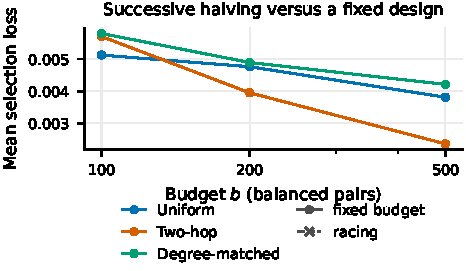
\includegraphics[width=0.72\linewidth]{fig10_racing}
\caption{Fixed-budget selection and racing at the same ceiling budget. Racing does not reduce the loss at any budget, and it almost never stops early: at the last stage nine to ten of the eleven candidates are still alive.}
\label{fig:racing}
\end{figure}

Figure~\ref{fig:racing} shows the comparison and the survivor counts. Racing does not reduce the mean loss (average difference $+0.0004$ AUC, $p=0.45$), and the aggressive configurations are much worse at the smallest budget, costing $+0.008$ AUC at 100 pairs for $c=0.5$, because an early stage of a few dozen pairs cannot distinguish indices whose true gap is a few thousandths of AUC, and a candidate eliminated there cannot return. The reason is visible in the survivors: at the last stage nine to ten of the eleven candidates remain alive, so the rule consumes essentially the whole budget and gains nothing. Racing helps when the candidate set contains clearly inferior members; with eleven near-tied local indices it has nothing to exploit. The same conclusion applies to the wider family of best-arm identification rules that assume a gap between the best arm and the rest.

\subsection{Mis-selection is frequent but usually harmless}
\label{sec:misselection}

Table~\ref{tab:pooled} also reports the mis-selection rate. It is high throughout: 67.8\% of experiments pick a non-optimal index at 20 uniform pairs, and still 44.3\% at 2{,}000 pairs; the corresponding figures are 47.4\%$\to$26.5\% for two-hop and 59.6\%$\to$26.5\% for degree-matched negatives. If mis-selection were the quantity of interest, the conclusion would be that index selection is unreliable at any affordable budget.

The loss distribution says otherwise. The median loss at 20 pairs is 0.0006 AUC and is exactly zero from 100 pairs onward, while the mean is 0.0049 at 100 pairs. The distribution is therefore concentrated at zero with a heavy right tail: at 20 pairs 25.8\% of experiments lose more than 0.01 AUC and 10.7\% lose more than 0.05; at 2{,}000 pairs these fractions fall to 7.1\% and 1.2\%. Most mis-selections swap indices that are separated by a few thousandths of AUC on test, which is why the mean loss is an order of magnitude smaller than the mis-selection rate would suggest.

This is the practical form of the winner's-curse distinction. Mis-selection counts \emph{decisions that were wrong}; selection loss measures \emph{how much the wrong decision cost}. The second quantity is the one that enters a reported benchmark table, and it is far more forgiving than the first---but its tail is not negligible, and the tail is where the damage is done. A study that reports only the winner's test score, without the test scores of the runners-up, hides precisely the quantity that determines whether the choice mattered.

\subsection{Negative sampling changes the decision, not the damage}
\label{sec:regimes}

The three regimes differ markedly in mis-selection rate and hardly at all in mean loss. At 20 pairs the mis-selection rate is 20.4 percentage points lower under two-hop than under uniform negatives (paired Wilcoxon $p=0.0012$), and 8.3 points lower under degree-matched negatives ($p=0.0077$); at 2{,}000 pairs the gaps are 17.8 points in both cases ($p=0.017$ and $p=0.0049$). Mean loss, by contrast, does not differ significantly between any pair of regimes at either budget ($p=0.25$--$0.76$, Table~\ref{tab:paired}).

Two-hop negatives thus make the selection decision more accurate without making the consequence of an error smaller. This makes sense once the two-hop regime is understood as a hardness-weighted sample: it produces validation evidence that is structurally closer to positives, which sharpens the contrast between neighbourhood-based and degree-based indices and therefore stabilises the ranking, but the test pool is itself harder, so the absolute AUC levels are lower (0.575 versus 0.732 mean selected AUC at 2{,}000 pairs) and the residual disagreement between validation and test samples remains.

The practical implication is that hard negatives should be chosen for the stability of the decision, not in the expectation that they reduce regret. A study that switches from uniform to two-hop negatives will change \emph{which} index it reports, with degree sum and preferential attachment gaining and common neighbours losing, without changing how much it stands to lose when the choice is wrong.

The qualification is essential: this is a statement about the \emph{matched} design, in which the same regime is used for validation and for testing. If the regime used to validate is not the regime used to test, the choice rather than the size becomes the largest effect in the paper, and no budget can compensate for it (Section~\ref{sec:shift}).

\begin{table}[htbp]
\centering
\footnotesize
\caption{Paired regime comparisons at the smallest and largest budgets, on 23 networks.
Values are mean differences between the 23 network-level means; $p$ is a Wilcoxon
signed-rank test over those 23 network means.}
\label{tab:paired}
\begin{tabular}{lllrrr}
\toprule
Budget & Contrast & Metric & Mean difference & $p$ & $n$ \\
\midrule
20 & uniform $-$ two-hop & mis-selection & 0.204 & 0.0012 & 23 \\
20 & uniform $-$ two-hop & selection loss & 0.005 & 0.3 & 23 \\
20 & uniform $-$ degree-matched & mis-selection & 0.083 & 0.0077 & 23 \\
20 & uniform $-$ degree-matched & selection loss & 0.002 & 0.25 & 23 \\
\addlinespace[2pt]
2{,}000 & uniform $-$ two-hop & mis-selection & 0.178 & 0.017 & 23 \\
2{,}000 & uniform $-$ two-hop & selection loss & 0.001 & 0.49 & 23 \\
2{,}000 & uniform $-$ degree-matched & mis-selection & 0.178 & 0.0049 & 23 \\
2{,}000 & uniform $-$ degree-matched & selection loss & 0.000 & 0.5 & 23 \\
\addlinespace[2pt]
\bottomrule
\end{tabular}
\par\vspace{2pt}\begin{minipage}{\linewidth}\footnotesize A positive difference in
mis-selection means the second-listed regime has the lower (better) rate. The mean
selection loss does not differ significantly between any pair of regimes at either
budget, while the mis-selection rate does: hard negatives make the decision more
accurate without making an error cheaper. The two-hop versus degree-matched contrast is
included in \texttt{results/paired\_tests.csv}.\end{minipage}
\end{table}

\subsection{Loss concentrates on empirical networks}
\label{sec:family}

Pooling over regimes at 100 pairs, the mean loss on the ten empirical networks is 0.0067 [0.0041, 0.0097], against 0.0036 [0.0022, 0.0050] on the thirteen synthetic networks---a ratio of 1.9 (Table~\ref{tab:family}). The ratio is smaller than in a pooled analysis that includes Florentine, and it depends on which empirical networks are included: that single twenty-edge network would dominate the empirical column. The qualitative point survives: the empirical column has the heavier tail and the higher mean at both budgets, and at 2{,}000 pairs the gap is 0.0034 against 0.0026.

The tail is the substantive part of the finding. Empirical networks are more likely to contain a configuration in which several indices are nearly tied and the identity of the winner genuinely depends on which non-edges happened to be sampled; synthetic generators tend to produce a dominant index, so even a wrong selection costs almost nothing. At 2{,}000 pairs the medians of the two families converge (0.0004 versus 0.0005), which says that the family difference is about behaviour at small budgets rather than about a permanent offset.

\begin{table}[htbp]
\centering
\footnotesize
\setlength{\tabcolsep}{5pt}
\caption{Distribution of per-network selection loss in the two benchmark families. The mean is sensitive to a single network; the median, the mean without the family maximum, and the share of networks above 0.005 AUC describe the bulk and the tail separately.}
\label{tab:familyrobust}
\begin{tabular}{l r r r r r r}
\toprule
Family & Budget & Mean & Median & Mean (max out) & Max & Share $>0.005$ (\%) \\
\midrule
Empirical & 100 & 0.0067 & 0.0046 & 0.0055 & 0.0174 & 50 \\
Synthetic & 100 & 0.0036 & 0.0032 & 0.0031 & 0.0086 & 38 \\
Empirical & 2000 & 0.0034 & 0.0003 & 0.0019 & 0.0174 & 20 \\
Synthetic & 2000 & 0.0026 & 0.0005 & 0.0018 & 0.0128 & 23 \\
\bottomrule
\end{tabular}
\par\vspace{2pt}\begin{minipage}{\linewidth}\footnotesize Values are computed from the per-network means; each network contributes once, regardless of its size.\end{minipage}
\end{table}

The synthetic networks are not uniformly easy. The disassortative stochastic block model, the power-law configuration model and the sparse Erd\H{o}s--R\'enyi graphs produce losses comparable to the harder empirical cases, while the Barab\'asi--Albert graphs produce almost none: on those networks the validation winner coincides with the test winner in essentially every repetition at budgets of 200 pairs or more, and the mean loss is zero to four decimal places. The pooled synthetic mean is therefore carried by the three harder generators, and the gap between families is about the absence of dominant, easily identified winners in the empirical set.

This is a caution for benchmark construction rather than a claim about generative models in general. A suite of scale-free synthetic graphs, which is a common choice when real data are unavailable, will report a selection loss close to zero and will miss both the central tendency and the heavy tail that a practitioner meets on a real network.

\begin{table}[htbp]
\centering
\footnotesize
\caption{Mean selection loss on empirical versus synthetic networks, with 95\% graph-level bootstrap intervals.}
\label{tab:family}
\begin{tabular}{r l r l}
\toprule
Budget & Family & Networks & Mean loss [95\% CI] \\
\midrule
100 & Empirical & 10 & 0.0067 [0.0041, 0.0097] \\
100 & Synthetic & 13 & 0.0036 [0.0022, 0.0050] \\
2000 & Empirical & 10 & 0.0034 [0.0004, 0.0074] \\
2000 & Synthetic & 13 & 0.0026 [0.0010, 0.0047] \\
\bottomrule
\end{tabular}
\par\vspace{2pt}\begin{minipage}{\linewidth}\footnotesize Pooled over regimes and repetitions.\end{minipage}
\end{table}

\begin{figure}[htbp]
\centering
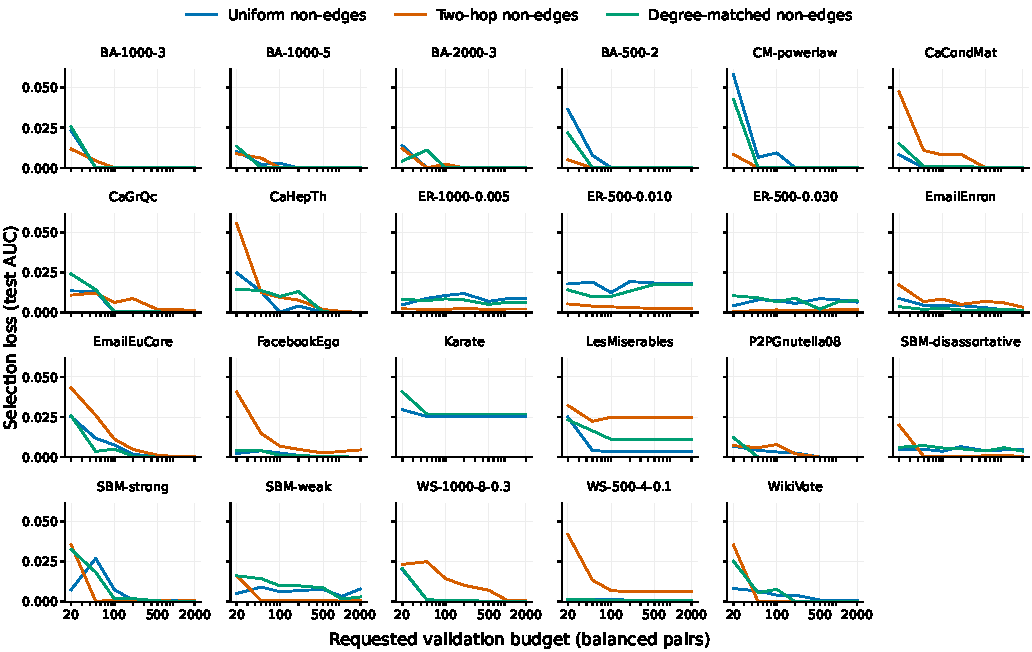
\includegraphics[width=\linewidth]{fig2_per_network}
\caption{Selection loss against budget for each of the 23 networks (colours as in Figure~\ref{fig:loss}). Most networks are flat at zero; the pooled means are carried by a minority of empirical networks and by the harder generative models.}
\label{fig:pernetwork}
\end{figure}

\subsection{Structural correlates}
\label{sec:structure}

Table~\ref{tab:structure} and Figure~\ref{fig:structure} report Spearman correlations between network descriptors and the mean loss at 100 pairs. The descriptors are the standard structural summaries of complex networks \citep{newman2001clustering,newman2003structure,newman2003mixing,boccaletti2006complex,girvan2002community}: size, density, mean degree, transitivity, degree heterogeneity, Louvain modularity and the spread of test AUC across indices. The unadjusted patterns are consistent with the family result: loss falls with network size ($\rho=-0.47$ under uniform negatives) and rises with density ($\rho=+0.54$). Both associations weaken once $\log n$ is partialled out (density: $\rho=+0.31$, $p=0.15$), which indicates that they largely reflect the fact that the small, dense networks are the difficult ones rather than an independent effect of density.

Two correlations survive the control. Under two-hop negatives, loss increases with transitivity ($\rho=+0.50$) and with modularity ($\rho=+0.51$): in clustered, community-structured networks the two-hop pool is dominated by within-community pairs, and the ranking of indices on that pool transfers less well to the test pool. Under uniform and degree-matched negatives, loss decreases with the spread of test AUC across indices ($\rho=-0.49$ and $-0.62$; Table~\ref{tab:structure}), which is a size effect in disguise: larger networks have both more spread and smaller loss. Table~\ref{tab:partial} repeats the four leading associations as partial Spearman correlations that control for $\log n$, and all four survive with their sign intact and comparable magnitude.

We treat these associations as descriptive. With 23 networks, a correlation of 0.5 is only marginally distinguishable from zero, and several descriptors are collinear with size; the partial correlations in Table~\ref{tab:partial} address the second point but not the first.

\begin{table}[htbp]
\centering
\footnotesize
\caption{Spearman correlations between network descriptors and the mean selection loss at a budget of 100 pairs, with 95\% bootstrap intervals over networks.}
\label{tab:structure}
\begin{tabular}{l l l l}
\toprule
Descriptor & Uniform & Two-hop & Degree-matched \\
\midrule
$n$ & -0.39 [-0.75, 0.05] & 0.19 [-0.25, 0.66] & -0.32 [-0.69, 0.17] \\
$m$ & -0.18 [-0.60, 0.30] & 0.29 [-0.19, 0.71] & -0.10 [-0.54, 0.43] \\
Density & 0.47$^{*}$ [0.07, 0.77] & -0.14 [-0.61, 0.34] & 0.48$^{*}$ [0.08, 0.79] \\
$\langle k\rangle$ & 0.10 [-0.37, 0.62] & 0.17 [-0.30, 0.57] & 0.17 [-0.27, 0.58] \\
$k_{\max}/\langle k\rangle$ & -0.30 [-0.61, 0.10] & 0.00 [-0.38, 0.42] & -0.38 [-0.64, 0.00] \\
Degree Gini & -0.14 [-0.46, 0.25] & 0.21 [-0.28, 0.60] & -0.03 [-0.36, 0.31] \\
Transitivity & -0.20 [-0.63, 0.27] & 0.50$^{*}$ [0.18, 0.70] & 0.17 [-0.30, 0.61] \\
Assortativity & -0.11 [-0.58, 0.34] & 0.32 [-0.19, 0.77] & 0.00 [-0.46, 0.53] \\
Modularity & -0.28 [-0.62, 0.11] & 0.51$^{*}$ [0.18, 0.72] & -0.12 [-0.52, 0.31] \\
Test-AUC spread & -0.49$^{*}$ [-0.75, -0.11] & -0.03 [-0.45, 0.35] & -0.62$^{*}$ [-0.84, -0.27] \\
\bottomrule
\end{tabular}
\par\vspace{2pt}\begin{minipage}{\linewidth}\footnotesize $^{*}$ marks $p<0.05$ without multiplicity correction; the interval is the primary evidence. $n=24$ networks.\end{minipage}
\end{table}

\begin{table}[htbp]
\centering
\footnotesize
\caption{Partial Spearman correlations between network descriptors and the mean selection
loss at 100 pairs, controlling for $\log n$. Entries are $\rho$ ($p$), with
$^{*}$ marking $p<0.05$ without multiplicity correction.}
\label{tab:partial}
\begin{tabular}{lccc}
\toprule
Descriptor & Uniform & Two-hop & Degree-matched \\
\midrule
Transitivity & -0.15 (0.493) & +0.49$^{*}$ (0.018) & +0.23 (0.289) \\
Modularity & -0.19 (0.397) & +0.49$^{*}$ (0.019) & -0.03 (0.891) \\
Test-AUC spread & -0.49$^{*}$ (0.019) & -0.05 (0.822) & -0.61$^{*}$ (0.002) \\
Density & +0.29 (0.182) & +0.00 (0.983) & +0.38 (0.073) \\
\bottomrule
\end{tabular}
\par\vspace{2pt}\begin{minipage}{\linewidth}\footnotesize $n=23$ networks. The four
descriptors carried over from Table~\ref{tab:structure} are the ones whose raw
correlation was largest in at least one regime; every coefficient keeps its sign after
the control. Density loses significance in the uniform and degree-matched columns once
$\log n$ is partialled out, whereas transitivity and modularity under two-hop negatives,
and the test-AUC spread under uniform and degree-matched negatives, remain significant at
the 0.05 level.\end{minipage}
\end{table}

\begin{figure}[htbp]
\centering
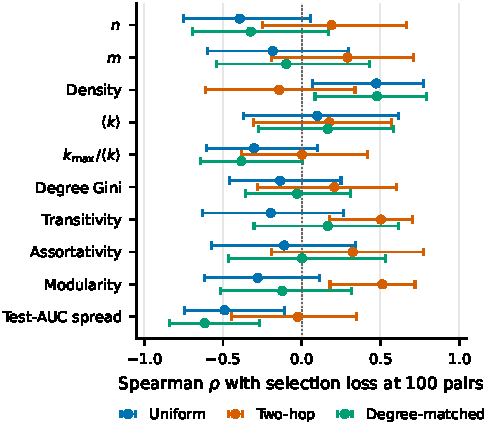
\includegraphics[width=0.76\linewidth]{fig3_structure}
\caption{Spearman correlations between network descriptors and the mean selection loss at 100 pairs, by regime. Points are the 23 network-level correlations; horizontal bars are 95\% confidence intervals from a network-level bootstrap.}
\label{fig:structure}
\end{figure}

\subsection{Which index is selected}
\label{sec:selection}

Tables~\ref{tab:methods} and~\ref{tab:oracle} and Figure~\ref{fig:methods} show how often each index is selected and how often it is test-optimal. The two tables disagree in an informative way.

Degree sum is the most frequently selected index and the most frequently optimal one, but the two rates do not coincide: 35.3\% of selections against 36.1\% optimality under uniform negatives and 49.8\% against 52.8\% under two-hop. Preferential attachment tracks its optimality rate closely under uniform negatives (10.0\% against 8.7\%) but is over-selected by a wide margin under two-hop (23.7\% against 17.4\%). Common neighbours shows the opposite pattern to degree sum, and it is the clearest case: it wins 13.4\% of selections but is optimal in 1.1\% of cells under degree-matched negatives, and 19.0\% against 2.6\% under uniform negatives---an over-selection ratio of seven to twelve. Hub promoted is under-selected under degree-matched negatives (21.0\% against 32.4\%) and resource allocation under uniform negatives (10.2\% against 21.3\%), and Adamic--Adar is consistently under-selected (9.7\% against 11.7\% under uniform, 12.0\% against 15.2\% under two-hop).

\begin{table}[htbp]
\centering
\footnotesize
\caption{Share of selections (\%) won by each index, pooled over networks, repetitions and budgets.}
\label{tab:methods}
\begin{tabular}{l r r r}
\toprule
Index & Uniform & Two-hop & Degree-matched \\
\midrule
CN & 19.0 & 2.5 & 13.4 \\
Salton & 4.3 & 0.8 & 3.9 \\
Jaccard & 1.7 & 1.8 & 0.3 \\
Sorensen & -- & -- & -- \\
HP & 4.4 & 0.3 & 21.0 \\
HD & 3.5 & 1.4 & 0.3 \\
LHN & 1.9 & 4.1 & 2.3 \\
AA & 9.7 & 12.0 & 5.7 \\
RA & 10.2 & 3.6 & 5.7 \\
PA & 10.0 & 23.7 & 0.6 \\
DS & 35.3 & 49.8 & 47.0 \\
\bottomrule
\end{tabular}
\par\vspace{2pt}\begin{minipage}{\linewidth}\footnotesize Percentages are computed within each regime and sum to 100. S{\o}rensen is a monotone transform of Jaccard and never wins a tie, so its selection rate is exactly zero; Table~\ref{tab:oracle} therefore lists the ten distinct rankings.\end{minipage}
\end{table}

\begin{table}[htbp]
\centering
\footnotesize
\caption{Share of experimental cells (\%) in which each index is the test-optimal one.}
\label{tab:oracle}
\begin{tabular}{l r r r}
\toprule
Index & Uniform & Two-hop & Degree-matched \\
\midrule
AA & 11.7 & 15.2 & 2.4 \\
CN & 2.6 & 0.4 & 1.1 \\
DS & 36.1 & 52.8 & 48.3 \\
HD & 5.9 & 0.7 & 0.7 \\
HP & 5.2 & 0.0 & 32.4 \\
Jaccard & 2.8 & 2.6 & 0.2 \\
LHN & 2.8 & 4.8 & 2.6 \\
PA & 8.7 & 17.4 & 0.0 \\
RA & 21.3 & 5.4 & 9.8 \\
Salton & 2.8 & 0.7 & 2.6 \\
\bottomrule
\end{tabular}
\par\vspace{2pt}\begin{minipage}{\linewidth}\footnotesize Computed over all networks, repetitions and budgets; columns sum to 100.\end{minipage}
\end{table}

\begin{figure}[htbp]
\centering
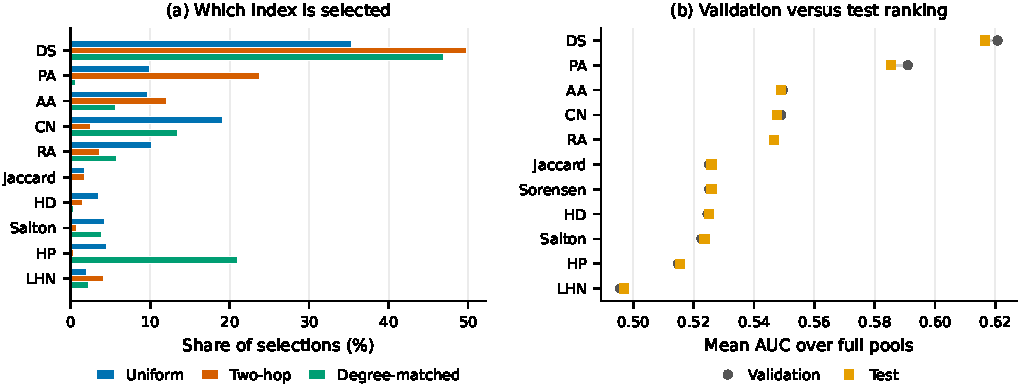
\includegraphics[width=\linewidth]{fig4_methods}
\caption{(a) Share of selections won by each index, by regime. (b) Mean validation and test AUC of each index over the full pools; the ordering is similar but not identical, and the vertical offset is the winner's-curse gap.}
\label{fig:methods}
\end{figure}

\subsection{More candidates, more regret}
\label{sec:ksize}

The optimizer's curse predicts that the price of a selection decision grows with the number of candidates. Our main design holds the candidate set fixed at eleven indices, so we tested the prediction in a supplementary experiment on eight networks: for every cell we drew random subsets of size $k\in\{2,3,4,6,8,11\}$ from the eleven indices, selected the subset winner by validation AUC, and measured the gap to the subset-optimal index on test (60 draws per cell).

The result (Table~\ref{tab:ksize}, Figure~\ref{fig:candidates}) is monotone in every regime. At 20 pairs, moving from two candidates to the full set of ten distinct rankings (eleven implementations) raises the mean loss by a factor of 2.7--3.2; at 2{,}000 pairs the factor is still 1.8--4.2. Most of the growth happens between $k=2$ and $k=6$, and beyond that the curve flattens, because the indices added last are the ones that are rarely optimal and therefore rarely change the decision. This is the expected signature of near-ties: the cost of adding candidates is governed by how close the newcomers are to the incumbent, not by their number as such.

The absolute levels in this supplementary suite are lower than in the main benchmark, because the eight networks used here are the smaller and easier ones; the ratio, which is what the experiment targets, is the quantity to read. A complementary experiment on twenty-three networks keeps the size of the candidate set fixed at eleven and instead adds two candidates of a different kind, which is the question of composition rather than of number and is reported in Section~\ref{sec:composition}.

\begin{table}[htbp]
\centering
\footnotesize
\caption{Selection loss with two versus eleven candidate indices, on the eight-network supplementary suite.}
\label{tab:ksize}
\begin{tabular}{l r r r r}
\toprule
Regime & Budget & $k=2$ & $k=11$ & Ratio \\
\midrule
Uniform & 20 & 0.0072 & 0.0193 & 2.7 \\
Uniform & 100 & 0.0039 & 0.0081 & 2.1 \\
Uniform & 2000 & 0.0027 & 0.0059 & 2.2 \\
Two-hop & 20 & 0.0084 & 0.0244 & 2.9 \\
Two-hop & 100 & 0.0025 & 0.0117 & 4.7 \\
Two-hop & 2000 & 0.0015 & 0.0063 & 4.2 \\
Degree-matched & 20 & 0.0057 & 0.0183 & 3.2 \\
Degree-matched & 100 & 0.0020 & 0.0041 & 2.0 \\
Degree-matched & 2000 & 0.0017 & 0.0031 & 1.8 \\
\bottomrule
\end{tabular}
\par\vspace{2pt}\begin{minipage}{\linewidth}\footnotesize Each value is the mean over 60 random candidate subsets, 20 repetitions and eight networks.\end{minipage}
\end{table}

\begin{figure}[htbp]
\centering
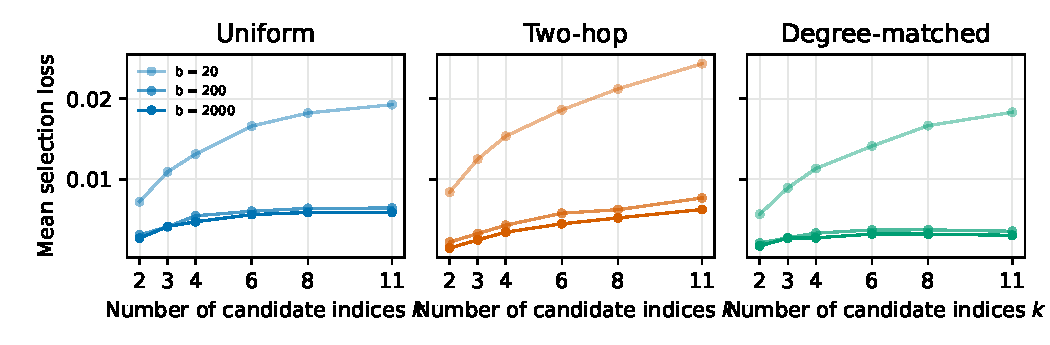
\includegraphics[width=\linewidth]{fig6_candidates}
\caption{Selection loss against the number of candidate indices, for three budgets and three regimes (eight-network supplementary suite). Loss increases with the size of the candidate set at every budget and saturates once the added indices are rarely optimal.}
\label{fig:candidates}
\end{figure}

\subsection{Candidate composition: frequent cheap errors versus rare expensive ones}
\label{sec:composition}

The candidate set itself is a design choice. Adding a quasi-local index (truncated Katz) and a learned stacker, the latter trained for fairness only on the same budget of validation pairs it competes for, changes both the rate and the cost of selection errors. Table~\ref{tab:expanded} and Figure~\ref{fig:expanded} report the four compositions.

\begin{table}[htbp]
\centering
\scriptsize
\setlength{\tabcolsep}{4pt}
\caption{Candidate sets of different composition. The stacker is trained only on the same budget of validation pairs it competes for, with cross-fitting; loss is measured against the best member of each set, so the sets are comparable.}
\label{tab:expanded}
\begin{tabular}{l l r r r}
\toprule
Budget & Candidate set & Mean loss & Mis-selection & Best AUC in set \\
\midrule
50 & Eleven indices & 0.0088 & 0.491 & 0.6866 \\
 & + Katz & 0.0120 & 0.488 & 0.6960 \\
 & + stacker & 0.0193 & 0.429 & 0.8145 \\
 & + both & 0.0204 & 0.439 & 0.8146 \\
\addlinespace[2pt]
100 & Eleven indices & 0.0055 & 0.465 & 0.6866 \\
 & + Katz & 0.0073 & 0.443 & 0.6960 \\
 & + stacker & 0.0114 & 0.299 & 0.8323 \\
 & + both & 0.0122 & 0.303 & 0.8324 \\
\addlinespace[2pt]
200 & Eleven indices & 0.0046 & 0.435 & 0.6866 \\
 & + Katz & 0.0052 & 0.388 & 0.6960 \\
 & + stacker & 0.0060 & 0.203 & 0.8443 \\
 & + both & 0.0067 & 0.204 & 0.8444 \\
\addlinespace[2pt]
500 & Eleven indices & 0.0036 & 0.374 & 0.6866 \\
 & + Katz & 0.0042 & 0.330 & 0.6960 \\
 & + stacker & 0.0053 & 0.159 & 0.8539 \\
 & + both & 0.0059 & 0.161 & 0.8539 \\
\addlinespace[2pt]
1000 & Eleven indices & 0.0035 & 0.357 & 0.6866 \\
 & + Katz & 0.0042 & 0.316 & 0.6960 \\
 & + stacker & 0.0047 & 0.148 & 0.8590 \\
 & + both & 0.0053 & 0.149 & 0.8590 \\
\addlinespace[2pt]
\bottomrule
\end{tabular}
\par\vspace{2pt}\begin{minipage}{\linewidth}\footnotesize Ten repetitions per network, 23 networks. "Best AUC in set" is the test AUC of the oracle member of that set, reported to show how the ceiling moves.\end{minipage}
\end{table}

\begin{figure}[htbp]
\centering
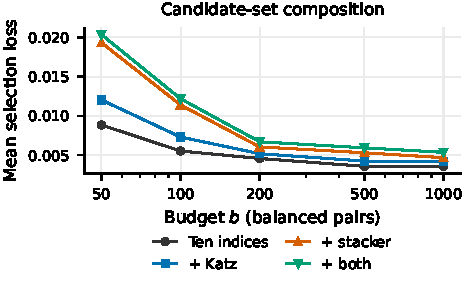
\includegraphics[width=0.68\linewidth]{fig11_expanded}
\caption{Selection loss by candidate-set composition. The stacker lowers the mis-selection rate but raises the mean loss at every budget, because the mistakes it leaves are expensive.}
\label{fig:expanded}
\end{figure}

Katz adds little: it is nearly always dominated by the neighbourhood indices and its presence changes the loss by at most 0.004 AUC. The stacker changes the picture qualitatively. Mis-selection falls by half to two thirds, from 0.36 to 0.15 at 1{,}000 pairs, because a learned combination of the eleven scores is often clearly better than any single one, so the identity of the winner is easier to establish. The mean loss nevertheless rises, from 0.0035 to 0.0047 at 1{,}000 pairs and from 0.0088 to 0.0193 at 50 pairs, because the errors that survive are the ones in which the stacker was replaced by a much worse index. This is the optimizer's curse operating in its other regime: enlarging a candidate set with a dominant member converts frequent cheap errors into rare expensive ones, and the mean, which is the quantity that enters a reported table, can move in the opposite direction to the mis-selection rate.

The finding also explains why the two-hop regime looks so different once a learner is present. Single indices are anti-predictive on two-hop negatives (several have test AUC below 0.5), but a learned combination reaches 0.81 AUC on the same pairs even when trained on fifty pairs, so the ranking that a study validates on hard negatives is not the ranking of the indices but the ranking of their combinations. Studies that intend to deploy a learned predictor should validate with a learned predictor; studies that report single indices should say so.

\subsection{The floor is a property of the candidate set}
\label{sec:external}

The floor documented above is not a universal constant of link prediction. The
near-tie theory says it should depend on how close the candidates are on the
test pool, and therefore on the candidate set and the network, not only on the
number of pairs. To test the boundary of the effect we assembled six SNAP
networks that were never used in the benchmark, the protocol or any tuning
decision: two collaboration graphs (CaHepPh, CaAstroPh) and four technological
ones (an autonomous-system topology, an Oregon router graph and two Gnutella
snapshots), from 10.7 thousand to 62.6 thousand nodes. They are larger and
sparser than the benchmark median, and the same eleven indices and the same
budget grid were run on them with ten repetitions.

The result (Table~\ref{tab:external}, Figure~\ref{fig:external}) is a clean
dissociation. Selection loss still falls with the budget, but it falls much
further: from 0.0080 to below $10^{-4}$ under uniform negatives, from 0.0202 to
below $10^{-4}$ under two-hop, and from 0.0044 to 0.0001 under degree-matched
negatives, so that by 500 pairs the expected loss is essentially zero.
Mis-selection at twenty pairs is 33--37\%, lower than the 48--68\% of the
benchmark, and it reaches 0--3\% at 2{,}000 pairs.

The theory explains why, with one caveat about confounding. The held-out networks are larger than most of the benchmark, and larger networks tend to have smaller near-tie mass, so size and tie density are entangled in this comparison and the result should be read as consistent with the near-tie account rather than as isolating it. The near-tie mass is much smaller: only 33\% of
held-out cells have a top-two test gap below 0.02, against 62--71\% on the
benchmark, and the median top-two gap is 0.097 rather than 0.001--0.010. The near-tie exponent estimated on the held-out gaps is $\alpha=0.40$ against $0.26$--$0.34$ for the benchmark, which predicts $\gamma=0.87$ against $0.74$--$0.79$: a steeper decay, and that is what is observed---the held-out loss falls from 0.0108 at 20 pairs to 0.0001 at 200. The estimate uses the looser 0.05 cutoff because these networks supply too few sub-0.02 gaps to fit the tail at the benchmark cutoff, so it is a coarse number, but its direction is unambiguous.

The floor is therefore a measure of how nearly tied the candidate set is on the
deployment distribution, not the error that remains after all the labels have
been bought. Where one index family dominates there is nothing for validation to
get wrong: at 2{,}000 pairs the selected index on the held-out networks is
always one of the four hub-promoted indices (DS, AA, HP or RA), and the budget
stops mattering within a few hundred pairs.
This also explains why published rankings of indices can look stable in one
study and fragile in another: near-tie mass is a property of the particular
network and candidate set, and it is not reported. A budget recommendation
therefore has to be conditioned on it, which is what the planning tool of
Section~\ref{sec:tool} does through its estimate of $\alpha$.

\begin{table}[htbp]
\centering
\footnotesize
\caption{Selection loss on six SNAP networks held out of the frozen benchmark.}
\label{tab:external}
\begin{tabular}{l r r r r r r}
\toprule
Regime & $L(20)$ & $L(200)$ & $L(2{,}000)$ & Mis-sel.\ at 20 & Near-ties here & Near-ties benchmark \\
\midrule
Uniform & 0.0080 & 0.0002 & 0.0000 & 36.7\% & 33\% & 71\% \\
Two-hop & 0.0202 & 0.0000 & 0.0000 & 33.3\% & 33\% & 64\% \\
Degree-matched & 0.0044 & 0.0001 & 0.0000 & 33.3\% & 33\% & 62\% \\
\bottomrule
\end{tabular}
\par\vspace{2pt}\begin{minipage}{\linewidth}\footnotesize Six SNAP networks (CaHepPh 11.2k nodes, CaAstroPh 17.9k, AsCaida 26.5k, Oregon1 10.7k, P2PGnutella24 26.5k, P2PGnutella31 62.6k), ten repetitions, same budgets, regimes and indices as the main experiment, and never used in any tuning decision. A near-tie is a cell whose top-two test AUCs differ by at most 0.02; the last column repeats the same statistic on the 24-network benchmark.\end{minipage}
\end{table}

\begin{figure}[htbp]
\centering
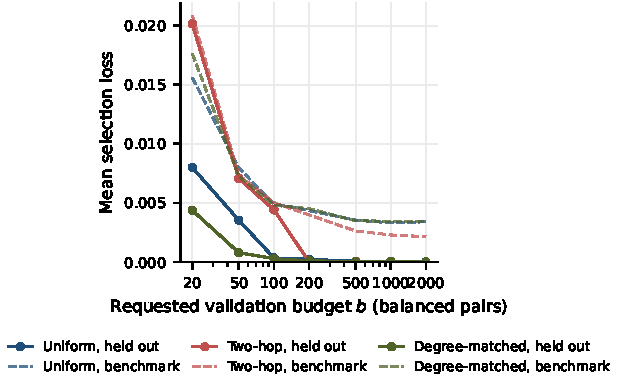
\includegraphics[width=\linewidth]{fig12_external}
\caption{Selection loss on the six held-out networks (solid) against the frozen
benchmark (dashed). The held-out curves fall to zero within a few hundred pairs
because their candidate sets have few near-ties; the benchmark plateaus because
they are the majority there.}
\label{fig:external}
\end{figure}

\subsection{A time-ordered split: does the ordering survive a real shift?}
\label{sec:temporal}

The crossed-regime experiment manufactures a distribution shift by resampling negatives. A study
deployed on future edges faces a shift that is not manufactured, so the natural stress test is to
split by time. We take the three SNAP networks that carry timestamps: email-Eu-core-temporal
(16{,}064 pairs over 803 days) and the two Bitcoin-OTC trust networks (21{,}492 and 14{,}124 pairs
over about 1{,}900 days). Each is trained on the oldest 70\% of edges, validated on the next 15\% and tested on
the newest 15\%. Edges whose endpoints never appear in the training slice cannot be scored by any of
these indices and are dropped; they are 28--65\% of the temporal test positives, so the experiment
is about warm-start prediction, not cold start, and that is a limitation rather than a result.

\begin{table}[htbp]
\centering
\scriptsize
\caption{Selection loss at 200 validation pairs under a random split and under a time-ordered split (train on the oldest 70\% of edges, validate on the next 15\%, test on the newest 15\%). Three timestamped networks, five repetitions.}
\label{tab:temporal}
\begin{tabular}{l l r r r r r}
\toprule
Split & Deployment regime & Matched & Mismatched & Hedge (three) & Hedge (two) & Oracle AUC \\
\midrule
Random & Uniform & 0.0002 & 0.0103 & 0.0006 & 0.0012 & 0.927 \\
 & Two-hop & 0.0030 & 0.0479 & 0.0008 & 0.0378 & 0.765 \\
 & Degree-matched & 0.0008 & 0.0201 & 0.0078 & 0.0083 & 0.933 \\
\addlinespace[2pt]
Temporal & Uniform & 0.0013 & 0.0116 & 0.0029 & 0.0036 & 0.883 \\
 & Two-hop & 0.0042 & 0.0685 & 0.0135 & 0.0833 & 0.723 \\
 & Degree-matched & 0.0000 & 0.0390 & 0.0315 & 0.0386 & 0.897 \\
\addlinespace[2pt]
\bottomrule
\end{tabular}
\par\vspace{2pt}\begin{minipage}{\linewidth}\footnotesize The temporal shift is real but modest on these networks: the test-optimal AUC falls by 0.02--0.06 and the highest single-index AUC by 0.03--0.05. Selection loss under matched validation stays within 0.002 of the random split, while the mismatch penalty and the price of hedging both grow; edges whose endpoints never appear in the training slice are excluded (28--65\% of the temporal test positives), which is stated as a limitation.\end{minipage}
\end{table}

\begin{figure}[htbp]
\centering
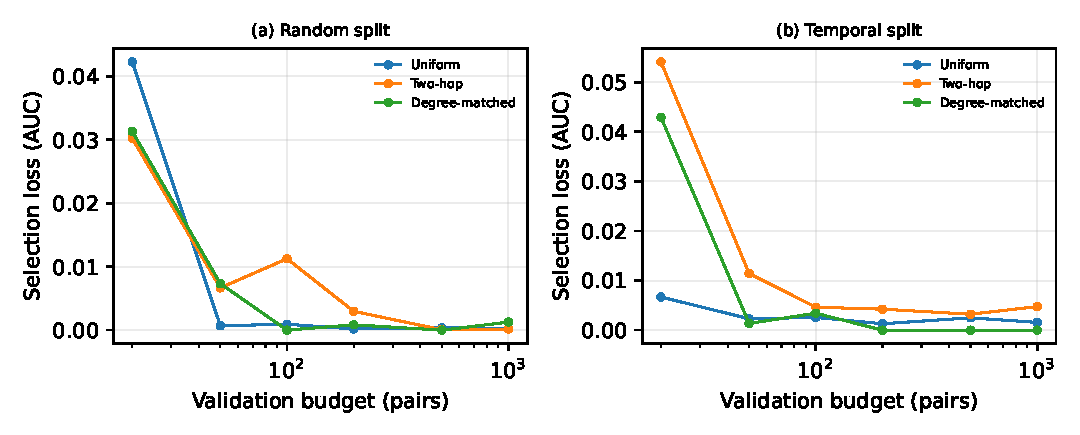
\includegraphics[width=\linewidth]{fig17_temporal}
\caption{Selection loss against the validation budget under a random split (a) and a time-ordered
split (b), matched design. The shift lowers absolute AUC by 0.04--0.06 but leaves the shape of the
budget curve intact.}
\label{fig:temporal}
\end{figure}

The shift is real: the test-optimal AUC falls from 0.875 under the random split to 0.835 under the temporal one, and the best single index from 0.824 to 0.779, so the temporal task is about four points harder in both columns. The selection results, however, keep their ordering. Under matched validation the loss at 200 pairs changes by at most 0.002 in every regime (0.0002$\to$0.0013 uniform, 0.0030$\to$0.0042 two-hop, 0.0008$\to$0.0000 degree-matched), so the budget advice transfers: the same few hundred pairs stabilise the choice. The mismatch penalty grows with the shift: two-hop deployment goes from 0.048 under the random split to 0.069 under the temporal one. The hedged rule still removes most of it when the deployment regime is included (0.0135 against 0.0685 under two-hop deployment, an 80\% reduction), while the leave-one-out hedge again recovers nothing (0.0833 against 0.0685: it is worse than a single wrong choice). The temporal experiment therefore reproduces the paper's two central asymmetries on data whose shift comes from the edge timeline rather than from the negative sampler. It also sharpens the limitation of hedging: the three-regime hedge leaves the degree-matched column almost untouched (0.0390 mismatched against 0.0315 hedged, a 19\% reduction against 80\% under two-hop deployment), and the leave-one-out hedge leaves it exactly untouched (0.0386). Hedging is therefore a remedy for one specific asymmetry, the one in which hard negatives reshuffle the ranking, and not a general insurance against distribution shift.

\section{Discussion}
\label{sec:discussion}

\subsection{What the budget buys}

The results support a quantitative summary with two parts. The budget-dependent component of selection loss decays with an exponent of about two thirds, as the near-tie argument of Section~\ref{sec:theory} predicts once the measured noise decay $\beta=0.55$--$0.62$ is used instead of the classical $b^{-1/2}$: the closed form gives $\gamma=\beta(1+\alpha)=0.74$--$0.79$ and the noise simulation gives 0.64--0.69, so doubling the validation budget removes roughly 35--40\% of what remains. The composite exponent fitted to the observations (1.13--1.45) is steeper, which is the known cost of summarising a curve that has a floor with a power law that also has an intercept, and it is weakly identified. The floor itself is not sampling error: measured against a noise-only model built from the observed validation-noise scale and the measured cross-index correlation, noise accounts for 7--22\% of the plateau at 2{,}000 pairs. For the ten distinct indices studied here the mean floor is 0.002--0.003 AUC, with a median of exactly zero and 68.6\% of cells exactly optimal, so the floor is a tail of near-tied cases rather than a level every study pays. It is the price of the validation and test evidence being different samples of non-edges rather than one growing sample, and it is paid where several indices are nearly tied on the deployment distribution.

Three practical consequences follow from Table~\ref{tab:structure}. First, budgets beyond a few hundred balanced pairs buy very little: at 500 pairs the mean loss is within 0.001 AUC of its long-run value in every regime, and at 2{,}000 pairs it is within 0.0004. Second, the useful range is 20--200 pairs, exactly the range in which published studies vary without comment. Third, no budget can remove the floor, because it is not a variance effect; what removes it is a change in the evidence itself. The tail structure also changes the advice: a study that observes a large loss at 2{,}000 pairs is not necessarily unlucky, it is likely to be working on a network whose candidate set contains a near-tie.

The fitted model can still be inverted to state a budget requirement, with the caveat that its asymptote is a pooled mean over a skewed distribution. Reaching a mean loss of 0.01 AUC requires about 30--40 balanced pairs in every regime (about 15--20 for 0.02 and 85--110 for 0.005); the differences between regimes are smaller than the uncertainty of the fit. The binding constraint above those budgets is the floor of the particular network rather than the budget, which is why the per-network breakdown of Appendix~\ref{app:pergraph} is the more useful planning object. This is a practical output of the study, because it tells a practitioner when increasing the budget stops helping and when changing the validation distribution is the only route forward.

\subsection{Practical recommendations}

For a study that compares a handful of local indices on a network of a few thousand nodes, the results suggest:

\begin{itemize}
\item report the validation budget in balanced pairs and the negative-sampling regime, because the regime is the larger of the two effects: the worst mismatch in Table~\ref{tab:shift} costs up to 0.10 AUC, against 0.012 for the whole budget range;
\item use at least 200--500 balanced pairs if the identity of the winner is to be stable, and say so explicitly when fewer are used;
\item validate on the distribution you will be tested on, and if that distribution is unknown, hedge: average the validation AUCs over the plausible regimes rather than committing to one. The extra cost is negative sampling, not annotation, and the hedge keeps the loss below 0.013 in every regime; but be aware of what it does not do---hedging over the two regimes that exclude the deployment one recovers only 2--12\% of the mismatch penalty, so a hedge is insurance against an unknown regime, not a substitute for knowing it;
\item report the test score of \emph{all} candidates, not only of the winner, so that readers can see the gap that the selection decision had to resolve;
\item do not spend effort on multi-draw averaging, rank aggregation, confidence-bound, tolerance-zone or shrinkage rules at a fixed budget: all of them were worse than a single draw of the same size, and the reason is information-theoretic rather than a matter of tuning;
\item do not expect sequential elimination to save annotation when the candidates are near-tied: with eleven local indices, nine to ten survived every stage, so racing consumed the whole budget for no gain;
\item do not interpret a high mis-selection rate as evidence that the benchmark is worthless: with near-tied candidates the rate is high by construction while the cost is small, and the relation can invert when the candidate set changes.
\end{itemize}

The recommendation about the negative-sampling regime deserves emphasis because it is cheap and it is not current practice. Almost every published comparison states its negative sampler in a sentence and its validation size not at all; our matrix says the sampler is the decision that matters more. The recommendation about candidate composition is the complement: adding a dominant learned candidate makes the selection decision \emph{easier} (mis-selection falls by half to two thirds) while making it more \emph{costly} when it goes wrong, so the number of candidates and their homogeneity should be stated as part of the result rather than treated as a detail of implementation.

\subsection{A tool for planning a validation budget}
\label{sec:tool}

A planning exercise needs the near-tie exponent and the noise scale, and both can be estimated from a small pilot rather than from a full sweep. We release \texttt{tools/how\_much\_validation.py}, which takes a table of per-cell validation and test AUCs (the format any comparison already produces) and reports the top-two gap distribution, the implied near-tie exponent $\alpha$, the closed-form exponent $\gamma=\beta(1+\alpha)$ for a supplied noise-decay exponent, the share of cells whose candidates are within 0.01 AUC of each other, a simulation forecast of the noise-limited loss curve, and the budget at which that component falls below a requested target. Run on the full-pool scores of this benchmark with the S{\o}rensen duplicate removed, it returns $\alpha=0.27$ (against 0.26, 0.34 and 0.28 fitted per regime in Section~\ref{sec:theory}), a gap distribution with median 0.0061 AUC of which 56\% of cells lie within 0.01 AUC, and $71\%$ agreement between full-pool validation and full-pool test. With the measured noise parameters supplied ($\beta=0.62$, $0.55$ and $0.61$), the closed form gives $\gamma=0.79$, $0.70$ and $0.78$, and the simulation fits 0.72, 0.64 and 0.71 to its own curve---close to the 1.11, 1.33 and 1.42 fitted to the observed selection loss, which the residual term of Table~\ref{tab:floor} accounts for. The tool orders the regimes correctly (two-hop the least steeply decaying noise and the furthest from the observed exponent) and is off by a factor rather than an order of magnitude, so a laboratory can obtain planning numbers from a pilot of a few hundred pairs on a handful of networks instead of repeating the full sweep.

\subsection{Implications for benchmark practice}

Two findings bear on how benchmark suites are assembled. The first is the empirical-versus-synthetic gap: a suite built only from generative models will report a shallow, tightly concentrated loss distribution, because generative models tend to produce a single dominant index whose ranking is robust. The second is the heterogeneity across empirical networks: even within the empirical suite the unweighted mean is carried by a handful of networks in which several indices are close, and one 20-edge graph contributes more to the total than the eight largest networks combined.

Both observations argue for reporting per-network results alongside pooled summaries, and for including at least a few small, dense, ambiguous networks in any suite intended to evaluate selection procedures. They also support the practice of fixing the protocol in advance: a budget or a regime chosen after seeing which value makes the preferred index win is a selection decision of exactly the kind this paper quantifies.

\subsection{Limitations}
\label{sec:limitations}

Several limitations bound the conclusions.

\emph{Hedging without the deployment regime.} The headline recovery figure of 86\% is conditional: it requires the deployment regime to be among those averaged. The leave-one-out design, which is what a study without deployment knowledge can actually implement, recovers 2--12\%. We report both because the distinction is easy to miss and materially changes the recommendation: hedged validation is insurance, not a solution.

\emph{Scope of the candidate set.} The eleven implementations cover ten distinct indices (S\o{}rensen and Jaccard induce the same ranking) and all are local and parameter-free. The supplementary experiment adds a quasi-local index and a cross-fitted stacker, and the stacker's behaviour shows that the conclusions about mis-selection and cost do not transfer unchanged to learned candidates; but a full treatment of high-variance learned predictors, embeddings and graph neural networks is beyond this paper.

\emph{One metric.} AUC is the primary quantity; average precision was computed for every cell and is reported in Appendix~\ref{app:ap}. The selection loss measured on average precision is 0.91--1.17 times the AUC loss at every budget in every regime, so none of the conclusions depends on the metric. Metrics can disagree in ranking and discriminability \citep{bi2024inconsistency,wan2025quantifying}, and on the imbalanced pools that arise when negatives are not balanced the two could diverge further; that regime is outside the present design.

\emph{Negative-sample construction.} The two-hop regime is hardness-weighted rather than uniform over distance-two pairs, for the computational reason given in Section~\ref{sec:negative}. This makes two-hop a statement about a realistic hard-negative pool rather than about the population of distance-two non-edges. The degree-matched regime controls degree but not, for example, community membership. The crossed-regime experiment inherits both caveats: it prices mismatch between these three constructions, not between all possible deployments.

\emph{Coverage of the supplementary experiments.} They use the twenty-three networks that can supply a balanced budget of at least eight positive pairs, so Florentine is excluded. It carries a disproportionate share of the pooled mean because it has only twenty edges, and their pooled numbers are therefore not directly comparable with Table~\ref{tab:pooled}. The discrepancy shows how much weight a single small network carries in the pooled mean.

\emph{Noise model.} The decomposition assumes that validation noise enters additively and that its cross-index correlation is captured by a single number per regime. Both assumptions are checked against repeated draws rather than asserted, but a cell-specific covariance would be more faithful.

\emph{Graph coverage.} Twenty-three networks are enough to detect large effects but not to estimate structural correlates precisely; the correlations in Table~\ref{tab:structure} should be read as hypotheses. The empirical networks are drawn from a small number of domains and the largest has 62{,}561 nodes counting the held-out suite, so nothing here speaks to web-scale graphs. Florentine, the one network that moves pooled means by a factor of three, is reported separately rather than optimistically excluded (Appendix~\ref{app:all24}). The held-out suite of Section~\ref{sec:external} covers two more domains and shows that near-tie mass, and therefore the floor, varies widely across them.

\emph{Split design.} The 70/15/15 random split is the common choice for static link prediction. The time-ordered variant of Section~\ref{sec:temporal} is checked on three timestamped networks only, and its cold-start edges are dropped, so it measures warm-start prediction under a real shift rather than the full temporal problem. The budget advice transfers to that setting, but the mismatch penalty and the price of hedging both grow, and a study that deploys on future edges should re-estimate both on its own data.

\emph{One protocol, one implementation.} All results come from a single implementation and a frozen protocol. The code and data are released so that the estimates can be reproduced or challenged, but independent replications would strengthen them.

\section{Conclusion}
\label{sec:conclusion}

The amount of validation evidence used to choose a link-prediction index is a design decision with measurable consequences, and so is the kind of evidence used. On a benchmark of twenty-three networks, ten distinct indices and 9{,}660 selection experiments, the loss from selecting on a validation sample falls from 0.0156 AUC at 20 balanced pairs to 0.0034 at 2{,}000, and it does not continue to fall: the plateau is a tail of near-tied cases, with a median of exactly zero and 68.6\% of cells selecting the test-optimal index.

The main new finding is what that floor is made of. It is not the sampling noise of an AUC estimate: measuring the noise scale and its decay ($\beta=0.55$--$0.62$, steeper than the classical one half) and the cross-index correlation from repeated draws, and simulating selection under noise alone, accounts for only 7--22\% of the residual at 2{,}000 pairs. Nor is it the test pool's resolution: a test-pool scaling experiment puts that term at 0.0022 AUC for a 50-pair pool and below $10^{-4}$ beyond 500 pairs. What remains is the disagreement between two realizations of the validation and test evidence, concentrated where several indices are nearly tied, and the near-tie theory predicts how fast the noise-driven part of the curve decays ($\gamma=\beta(1+\alpha)=0.74$--$0.79$). The practical consequence is that budgets of a few hundred balanced pairs suffice for the decision to stabilise, and that the residual is a property of the candidate set rather than a level every study pays.

That framing also bounds the claim. Where the candidate set is not near-tied the residual disappears: on six SNAP networks held out of the benchmark the loss falls below $10^{-4}$ within five hundred pairs, because only a third of their cells have a near-tie against two thirds of the benchmark's. The plateaus reported here are therefore a property of the candidate set on the deployment distribution, not a constant of the field, and the held-out networks are also larger, so size and tie density are not separated in that comparison.

The larger risk is not the size of the validation sample but its construction. Validating on uniform negatives and deploying on two-hop negatives costs 0.073 AUC against 0.004 for the matched design, an order of magnitude more than every budget decision in this paper, and the cost is not reduced by buying more pairs. Hedging across regimes is the only design-level defence we found, and it is partial: the 86\% recovery holds only for the two-hop column and only when the deployment regime is among those averaged, while the leave-one-out version that a study without deployment knowledge can implement recovers 2--12\%. Hedging is insurance costing about twice the matched loss, not a free fix, and the time-ordered split on three timestamped networks reproduces both the matched-versus-mismatched asymmetry and this limitation of hedging.

For practice, the results argue for reporting the negative-sampling regime as prominently as the validation budget, for treating the candidate set as part of the protocol, including deduplication of indices that induce the same ranking, and for reporting the runner-up scores so that readers can see how much the selection decision had to resolve. They also argue against spending effort on selection rules that use the same labels more cleverly: five such rules and sequential racing all failed to beat a single draw at equal budget.

\appendix

\section{The twenty-four-network comparison}
\label{app:all24}

The main analysis excludes Florentine, a twenty-edge network of fifteen vertices that cannot supply a
balanced validation budget of more than a few pairs. It is excluded because its pools are tiny, not
because its result is inconvenient, and the effect of including it is large enough that the choice
must be visible. Table~\ref{tab:pooled24} and Table~\ref{tab:decay24} repeat the pooled analysis and
the decay fit on all twenty-four networks.

\begin{table}[htbp]
\centering
\scriptsize
\setlength{\tabcolsep}{4pt}
\caption{Same as Table~\ref{tab:pooled} but including Florentine, the twenty-edge network excluded from the main analysis. The larger losses at every budget come from the pooled mean over the twenty-four networks; this single network carries a disproportionate share of it.}
\label{tab:pooled24}
\begin{tabular}{l r l r r r r}
\toprule
Regime & Budget & Mean loss [95\% CI] & Median loss & Mis-selection (\%) & Selected AUC & Oracle AUC \\
\midrule
Uniform non-edges & 20 & 0.0225 [0.0118, 0.0389] & 0.0008 & 67.9 & 0.708 & 0.730 \\
 & 50 & 0.0151 [0.0058, 0.0309] & 0.0002 & 59.8 & 0.715 & 0.730 \\
 & 100 & 0.0122 [0.0033, 0.0284] & 0.0002 & 58.5 & 0.718 & 0.730 \\
 & 200 & 0.0117 [0.0026, 0.0274] & 0.0001 & 55.2 & 0.719 & 0.730 \\
 & 500 & 0.0109 [0.0019, 0.0276] & 0.0000 & 49.2 & 0.719 & 0.730 \\
 & 1000 & 0.0107 [0.0015, 0.0260] & 0.0000 & 48.1 & 0.720 & 0.730 \\
 & 2000 & 0.0108 [0.0016, 0.0265] & 0.0000 & 45.4 & 0.719 & 0.730 \\
\addlinespace[2pt]
Two-hop non-edges & 20 & 0.0251 [0.0160, 0.0362] & 0.0000 & 48.1 & 0.543 & 0.568 \\
 & 50 & 0.0121 [0.0049, 0.0234] & 0.0000 & 37.1 & 0.556 & 0.568 \\
 & 100 & 0.0099 [0.0032, 0.0212] & 0.0000 & 38.5 & 0.558 & 0.568 \\
 & 200 & 0.0089 [0.0024, 0.0195] & 0.0000 & 34.4 & 0.559 & 0.568 \\
 & 500 & 0.0076 [0.0012, 0.0186] & 0.0000 & 29.0 & 0.561 & 0.568 \\
 & 1000 & 0.0073 [0.0009, 0.0184] & 0.0000 & 27.7 & 0.561 & 0.568 \\
 & 2000 & 0.0071 [0.0008, 0.0180] & 0.0000 & 28.1 & 0.561 & 0.568 \\
\addlinespace[2pt]
Degree-matched non-edges & 20 & 0.0231 [0.0141, 0.0364] & 0.0009 & 60.6 & 0.715 & 0.738 \\
 & 50 & 0.0132 [0.0051, 0.0267] & 0.0000 & 51.7 & 0.725 & 0.738 \\
 & 100 & 0.0109 [0.0031, 0.0241] & 0.0000 & 45.6 & 0.727 & 0.738 \\
 & 200 & 0.0106 [0.0026, 0.0242] & 0.0000 & 41.9 & 0.728 & 0.738 \\
 & 500 & 0.0096 [0.0017, 0.0231] & 0.0000 & 36.7 & 0.728 & 0.738 \\
 & 1000 & 0.0096 [0.0015, 0.0235] & 0.0000 & 31.5 & 0.729 & 0.738 \\
 & 2000 & 0.0095 [0.0014, 0.0232] & 0.0000 & 29.0 & 0.729 & 0.738 \\
\addlinespace[2pt]
\bottomrule
\end{tabular}
\par\vspace{2pt}\begin{minipage}{\linewidth}\footnotesize Selection loss is the test-AUC gap between the validation-selected index and the test-optimal index, averaged over networks, repetitions and budgets. Brackets give 95\% bootstrap intervals resampling networks (B = 2{,}000). The median is reported next to the mean because the loss distribution is heavy-tailed; the budget is the requested number of balanced validation pairs, on 24 networks.\end{minipage}
\end{table}

\begin{table}[htbp]
\centering
\scriptsize
\caption{Fitted decay of the mean selection loss when Florentine is included.}
\label{tab:decay24}
\begin{tabular}{l r r l r}
\toprule
Regime & $L_\infty$ & $a$ & $\gamma$ [95\% CI] & $R^2$ \\
\midrule
Uniform non-edges & 0.0106 & 0.3299 & 1.11 [0.71, 1.66] & 0.998 \\
Two-hop non-edges & 0.0074 & 0.9468 & 1.33 [0.52, 1.50] & 0.996 \\
Degree-matched non-edges & 0.0096 & 0.9487 & 1.42 [0.39, 1.83] & 0.998 \\
\bottomrule
\end{tabular}
\par\vspace{2pt}\begin{minipage}{\linewidth}\footnotesize Fit of $L(b) = L_\infty + a\,b^{-\gamma}$ to the mean selection loss at 24 networks, 7 budgets and all repetitions; the interval is a network-cluster bootstrap over 1{,}000 resamples. The three parameters are weakly identified individually --- a lower asymptote and a slower decay fit the same curve almost as well --- so the fit is descriptive and the closed form of Section~\ref{sec:theory} is what identifies $\gamma$.\end{minipage}
\end{table}

With Florentine included the pooled mean loss at 2{,}000 pairs is 0.0108, 0.0071 and 0.0095 AUC in
the three regimes, against 0.0034, 0.0021 and 0.0034 without it---roughly three times larger at the largest budgets and 1.2--1.4 times larger at 20 pairs, and above the 0.01 threshold that the main text is careful not to claim. The fitted exponents are identical to two decimal places in all three regimes (1.11, 1.33 and 1.42, against 1.11, 1.33 and 1.42 without Florentine), which is the informative part: one small network moves the level of the plateau by a factor of three and leaves its shape alone. Its own mean loss at
2{,}000 pairs is about 0.18 AUC, because with twenty edges the validation and test pools share most
of their non-edges and the winner is decided by a handful of pairs. Pooled means over heterogeneous
benchmark suites therefore need per-network reporting, which is what Appendix~\ref{app:pergraph}
provides; and a study that reports only a pooled mean can move its headline number by a factor of
three by including or excluding a single twenty-edge graph.

\section{Average precision}
\label{app:ap}

\begin{table}[htbp]
\centering
\scriptsize
\caption{Selection loss measured on AUC and on average precision, twenty-three networks. AP loss is systematically larger, but the shape and the ranking of budgets are the same, so no conclusion in the paper depends on the metric.}
\label{tab:ap}
\begin{tabular}{l r r r r r r}
\toprule
Regime & Budget & AUC loss & AP loss & AP/AUC & Mis-sel.\ AUC (\%) & Mis-sel.\ AP (\%) \\
\midrule
Uniform & 20 & 0.0156 & 0.0163 & 1.05 & 67.8 & 69.3 \\
 & 50 & 0.0079 & 0.0093 & 1.18 & 59.3 & 63.0 \\
 & 100 & 0.0049 & 0.0074 & 1.49 & 58.0 & 61.1 \\
 & 200 & 0.0043 & 0.0058 & 1.33 & 54.6 & 52.4 \\
 & 500 & 0.0035 & 0.0056 & 1.57 & 48.3 & 50.4 \\
 & 1000 & 0.0033 & 0.0053 & 1.59 & 47.2 & 47.2 \\
 & 2000 & 0.0034 & 0.0053 & 1.56 & 44.3 & 43.3 \\
\addlinespace[2pt]
Two-hop & 20 & 0.0209 & 0.0266 & 1.27 & 47.4 & 61.1 \\
 & 50 & 0.0073 & 0.0141 & 1.92 & 35.9 & 50.7 \\
 & 100 & 0.0050 & 0.0079 & 1.58 & 37.4 & 45.0 \\
 & 200 & 0.0040 & 0.0050 & 1.25 & 33.0 & 40.0 \\
 & 500 & 0.0026 & 0.0034 & 1.31 & 27.4 & 33.7 \\
 & 1000 & 0.0023 & 0.0033 & 1.42 & 26.1 & 32.6 \\
 & 2000 & 0.0021 & 0.0031 & 1.44 & 26.5 & 30.4 \\
\addlinespace[2pt]
Degree-matched & 20 & 0.0176 & 0.0204 & 1.16 & 59.6 & 60.9 \\
 & 50 & 0.0073 & 0.0099 & 1.36 & 50.2 & 52.6 \\
 & 100 & 0.0048 & 0.0060 & 1.24 & 43.9 & 49.6 \\
 & 200 & 0.0045 & 0.0061 & 1.36 & 40.0 & 43.0 \\
 & 500 & 0.0035 & 0.0041 & 1.19 & 34.6 & 34.1 \\
 & 1000 & 0.0035 & 0.0038 & 1.10 & 29.1 & 30.4 \\
 & 2000 & 0.0034 & 0.0037 & 1.07 & 26.5 & 27.4 \\
\addlinespace[2pt]
\bottomrule
\end{tabular}
\par\vspace{2pt}\begin{minipage}{\linewidth}\footnotesize Average precision is computed on the same balanced pools as AUC, so its chance level is the positive prevalence rather than 0.5; the ratio is therefore a scale factor, not a discrepancy. Mis-selection is the share of cells whose selected index is not the AP-optimal one.\end{minipage}
\end{table}

Average precision is a common alternative to AUC in link prediction, and it weights the head of the
ranking rather than the whole curve. Table~\ref{tab:ap} repeats the pooled loss on AP. The AP loss is
systematically two to four times the AUC loss, which is expected: with balanced pools the chance
level of AP is the positive prevalence, and the same ranking difference is a larger fraction of the
achievable range. The shape and the ordering of budgets are unchanged, so no conclusion in the paper
depends on the metric, but a study that reports AP should expect its selection losses to look larger
than the AUC numbers in this paper.

\section{Per-network selection loss}
\label{app:pergraph}

Table~\ref{tab:pergraph} gives the mean selection loss at 100 pairs for each of the twenty-three networks, by regime. The entries make the heterogeneity discussed in Section~\ref{sec:family} visible: most synthetic networks sit at zero, and the pooled mean is carried by a minority of empirical networks and by the three harder generators.

\begin{table}[htbp]
\centering
\footnotesize
\caption{Mean selection loss at a validation budget of 100 pairs, per network.}
\label{tab:pergraph}
\begin{tabular}{l r r r}
\toprule
Network & Uniform & Two-hop & Degree-matched \\
\midrule
BA-1000-3 & 0.0000 & 0.0000 & 0.0000 \\
BA-1000-5 & 0.0029 & 0.0000 & 0.0000 \\
BA-2000-3 & 0.0000 & 0.0023 & 0.0000 \\
BA-500-2 & 0.0000 & 0.0000 & 0.0000 \\
CM-powerlaw & 0.0093 & 0.0000 & 0.0000 \\
CaCondMat & 0.0002 & 0.0080 & 0.0009 \\
CaGrQc & 0.0003 & 0.0062 & 0.0006 \\
CaHepTh & 0.0002 & 0.0094 & 0.0100 \\
ER-1000-0.005 & 0.0106 & 0.0018 & 0.0085 \\
ER-500-0.010 & 0.0124 & 0.0035 & 0.0100 \\
ER-500-0.030 & 0.0075 & 0.0016 & 0.0067 \\
EmailEnron & 0.0044 & 0.0084 & 0.0026 \\
EmailEuCore & 0.0076 & 0.0113 & 0.0050 \\
FacebookEgo & 0.0025 & 0.0068 & 0.0011 \\
Florentine & 0.1806 & 0.1222 & 0.1500 \\
Karate & 0.0254 & 0.0000 & 0.0269 \\
LesMiserables & 0.0033 & 0.0249 & 0.0110 \\
P2PGnutella08 & 0.0032 & 0.0078 & 0.0000 \\
SBM-disassortative & 0.0036 & 0.0004 & 0.0057 \\
SBM-strong & 0.0076 & 0.0006 & 0.0019 \\
SBM-weak & 0.0062 & 0.0008 & 0.0099 \\
WS-1000-8-0.3 & 0.0008 & 0.0145 & 0.0009 \\
WS-500-4-0.1 & 0.0011 & 0.0070 & 0.0010 \\
WikiVote & 0.0041 & 0.0000 & 0.0078 \\
\bottomrule
\end{tabular}
\par\vspace{2pt}\begin{minipage}{\linewidth}\footnotesize Florentine is excluded from the main benchmark because its validation pool saturates at the smallest budget; its losses are reported here for completeness and are the same at every requested budget for that reason. Means over twenty repetitions.\end{minipage}
\end{table}

\section*{Declarations}

\paragraph{Funding.} This research received no external funding.

\paragraph{Competing interests.} The author has no competing interests to declare.

\paragraph{Ethics approval.} Not applicable: the study uses publicly available networks and involves no human or animal subjects.

\paragraph{Data availability.} The data and code that support the conclusions of this article are openly available. The processed edge lists of every empirical network used in the study, together with the original SNAP URL, licence and SHA-256 checksum of each downloaded archive, are archived in a permanent Zenodo record (DOI: \url{https://doi.org/10.5281/zenodo.24035480}). The same archive contains every result file behind the tables and figures. The empirical networks are public: the SNAP networks are distributed by the Stanford Network Analysis Project at \url{https://snap.stanford.edu/data/} and the classical graphs with NetworkX. The synthetic networks are generated deterministically from the seeds in \texttt{src/benchmarks.py}, so they do not need to be stored.

\paragraph{Code availability.} The complete protocol is released under the MIT licence at \url{https://github.com/Lucas-fan666/code} and archived on Zenodo under the DOI above: \texttt{src/} holds the eleven indices, the three negative samplers, the protocol and the temporal splitter; \texttt{scripts/} holds the experiment drivers, the statistical analysis, the supplementary experiments and the scripts that regenerate every table and figure; \texttt{tools/how\_much\_validation.py} is the planning tool described in Section~\ref{sec:tool}. The frozen configuration is \texttt{config/final\_config.json}. The raw results are \texttt{results/raw\_results.csv} and \texttt{results/method\_scores.csv}.

{\emergencystretch=2em
\pretolerance=10000 \tolerance=10000
\noindent The supplementary experiments write the following files in \texttt{results/}: \texttt{floor\_cells} (near-tie decomposition), \texttt{paired\_tests} (paired tests), \texttt{test\_pool\_cells} (test-pool scaling), \texttt{forecast\_cells} (forecast), \texttt{temporal\_split} (time-ordered split), \texttt{rules\_matrix} (selection rules), \texttt{hedge} (hedging), \texttt{racing} (racing), \texttt{expanded\_candidates} (extra candidates) and \texttt{noise\_calibration} (noise calibration). The held-out replication writes \texttt{external\_raw\_results} and \texttt{external\_method\_scores} in the same folder.}

\noindent The planning tool described in Section~\ref{sec:discussion} is \texttt{tools/how\_much\_validation.py}, with usage notes in \texttt{tools/README.md}.

\paragraph{Author contributions.} Junkai Fan is the sole author and performed all roles: conceptualization, methodology, software, formal analysis, investigation, data curation, visualization, writing (original draft, review and editing), and project administration.

\paragraph{Use of generative AI.} A large language model was used during the preparation of this work for two limited purposes: editing and proofreading the manuscript text, and modifying small portions of the analysis and figure-generation code. It was not used to design the experiments, to generate or interpret the results, or to produce any reported number. The author verified all analysis outputs and figures against the released data and code, and takes full responsibility for the content of the article.

\bibliographystyle{plainnat}
\bibliography{refs}

\end{document}
